\documentclass[12pt]{report}

\usepackage[utf8]{inputenc}
\usepackage[T1]{fontenc}
\usepackage[francais]{babel}
\usepackage{alltt}
\usepackage[top=2cm, bottom=2cm, left=3cm, right=3cm]{geometry}
\usepackage{graphicx} 
\usepackage{eurosym}
\usepackage[toc,page]{appendix}
\usepackage{setspace}
\usepackage{titlesec, color}
\usepackage{float}
\definecolor{gray75}{gray}{0.75}
\newcommand{\hsp}{\hspace{20pt}}
\titleformat{\chapter}[hang]{\Huge\bfseries}{\thechapter\hsp\textcolor{gray75}{|}\hsp}{0pt}{\Huge\bfseries}

\onehalfspacing

\begin{document}
%page de garde

  \vfill
\begin{minipage}{0.5\textwidth}
  Christophe \bsc{Blefari}\\
  Matthieu \bsc{Coelho}\\
  Clément \bsc{Daubigney}\\
  Thibaut \bsc{Zonca}\\
\end{minipage}

\vfill
  \hrule height 1.5pt
  \vskip 1cm
   \begin{center}
       {\Huge \textbf{Rapport final de projet industriel}} \\
       \vspace{0.5cm}
       \textsc{Création d'un tableau de bord interactif pour VMProject}\\
    \vspace{0.2cm} 
 
      

  \vskip 0.5cm
       
\includegraphics[width=0.35\textwidth]{pictures/versusmind.png}
      \hspace{5cm}
      
\includegraphics[width=0.25\textwidth]{pictures/esial.png}\\
  \vskip 1cm
  \hrule height 1.5pt
  
\end{center}
\vfill
\newpage{}

\chapter*{Remerciements}

Loin d'avoir été développé en solitaire, ce projet industriel a été réalisé en étroite collaboration avec l'entreprise VersusMind. C'est pourquoi nous tenons tout d'abord à les remercier pour avoir choisi notre équipe comme maître d'oeuvre du projet qu'ils proposaient et de nous avoir fait confiance. Leur présence, leur aide et leur compréhension nous a permis de travailler à notre rythme tout en respectant les objectifs fixés et d'avoir l'entrain pour mener à bien ce projet. Nous remercions donc tout particulièrement Benoit Zohar et Maxime Riggi, nos encadrants industriels, ainsi que Benoit Koch, le chef de l'entreprise. Nous adressons également une pensée à Assuntina Gessa, Jeoffrey Bauvin et Julie Pavillon, qui sont intervenus pour le bon déroulement de notre projet.\\

Les projets industriels sont des rencontres entre étudiants et entreprises mais également notre école, TELECOM Nancy, sans qui cette rencontre et plus globalement cette expérience ne serait pas possible. Nous tenons donc à apporter des remerciements à tous ceux qui, à TELECOM Nancy, font en sorte que le projet industriel puisse se réaliser, et tout particulièrement à Bertrand Petat pour son investissement et son encadrement. Nous n'oublions évidemment pas nos deux encadrantes universitaires, représentantes de l'école, Marie-Noëlle Flavenot et Marie-Claire Césare, qui ont été derrière nous pendant toute la durée du projet et qui ont su nous soutenir, nous motiver, nous aiguiller et nous conseiller en particulier dans les moments de doute. Elles ont donné de leur temps et de leur expérience pour nous aider à mener à bien notre projet.\\

Enfin nous remercions nos familles, nos proches et amis, pour leur soutien sans faille, et qui ont été présents lorsque nous avons eu besoin d'eux.\\

\tableofcontents
\listoffigures


\chapter*{Introduction}
\addcontentsline{toc}{chapter}{Introduction}

Le projet industriel de dernière année à TELECOM Nancy est un projet nécessaire pour l’obtention du diplôme. Il permet, à travers des outils vus en cours dans différents modules comme la gestion de projet, ou la programmation dans de multiples langages, de démontrer les capacités des l'élèves à mener à bien un projet informatique au sein d'une équipe.\\

Les projets sont proposés par des entreprises qui en font la demande auprès de l’établissement. Ils sont donc des objectifs réels pour les industriels, ce qui implique un contrat entre les deux parties. Des entretiens ont lieu ensuite entre les équipes intéressées et les industriels afin de sélectionner une équipe pour chaque projet.\\

VersusMind, un éditeur de logiciels, a développé un logiciel de gestion de projet en ligne : VMProject. Cette entreprise a proposé un sujet qui consiste à développer un nouveau tableau de bord pour ce logiciel. Le but est de permettre aux clients de VMProject d’avoir une vision globale de l’état actuel d’un ou plusieurs projets en cours, à l’aide de différent graphique sélectionnée auparavant, pour permettre la prise de décision. Nous nous sommes intéressé à ce projet, car il permet non seulement de développer nos compétence technique, mais aussi managérial. En effet savoir qu’elle type de données un chef de projet à besoin pour prendre des décisions est important. C’est donc ce projet qui a été confié à notre équipe, et nous mettons tout en œuvre pour le mener à terme.\\

\chapter{VersusMind, la société}

  \section{Présentation de l'entreprise}
  
VersusMind est un cabinet d’architecture numérique et un éditeur de logiciels innovants. Cette entreprise a été créée en 2006 par Benoit Koch, qui en est toujours à la tête actuellement, et est basée à Nancy. Elle compte au jour d’aujourd’hui vingt-cinq employés.\\

VersusMind propose des solutions exclusivement numériques, issues des technologies et de l’innovation. Grâce à une expertise en architecture technique, en communication interactive et en infrastructure de production, cette entreprise intervient sur l’ensemble de la chaîne de production. VersusMind repose sur trois piliers : \\

\begin{itemize}
\item L’indépendance vis-à-vis des éditeurs : les clients sont conseillés dans leurs choix avec étique et neutralité
\item La veille technologique : une veille intelligente est maintenue afin de forger l’expertise
\item La pérennité : les dispositifs mis en place sont efficaces à long terme\\
\end{itemize}

Afin de réussir les projets, les équipes de VersusMind sont pluridisciplinaires, complémentaires, décloisonnées et partageant la même vision. Ainsi, les effectifs de l’entreprise se composent aussi bien d’ingénieurs juniors ou seniors, d’architectes, ou encore de chefs de projets. Ces équipes travaillent généralement selon des méthodes agiles (Scrum particulièrement) ; pour cela, les équipes sont mises en avant et doivent primer sur les processus et les outils. De plus, le développement en soit d’une application est prioritaire par rapport à une documentation exhaustive. La collaboration avec le client est primordiale également, et comme tout processus agile, le changement est pris en compte et privilégié. Ces équipes pratiquent également le conseil pour accompagner les clients à chaque étape de leurs projets, selon plusieurs modèles : \\

\begin{itemize}
\item Stratégie Digitale : Aide à la définition d’une stratégie digitale complète.
\item Les tests de montée en charge ou encore la définition d’architecture physique en fonction de la montée en charge des sites.
\item Aide au démarrage : identification des points critiques, moyens techniques à mettre en œuvre, méthodologie.
\item Architecture : préconisations et définition du socle applicatif : schéma, intégration de librairies tierces, urbanisation.
\item Accompagnement : proof-of-concept, expertise, support technique, contrôle qualité du code, best-practices...\\
\end{itemize}
  
Ainsi, VersusMind se divise en trois divisions fortement imbriquées : le cabinet d’architecture numérique, l’agence, et VMSoftware.\\

		\subsection{Le cabinet d'architecture numérique}
	
\begin{figure}[!h]
	
\includegraphics[width=0.5\textwidth]{pictures/cabinet.png}
\end{figure}

VersusMind est un cabinet de Conseil en architecture technique mais également un intégrateur spécialisé dans la conception de projets numériques à haute valeur ajoutée. Cette entreprise possède deux domaines d’intervention, à savoir la réalisation de projets numériques et le conseil aux directions des systèmes d’informations. Les consultants interviennent dans les deux domaines, et peuvent : \\

\begin{itemize}
\item Proposer des recommandations fonctionnelles 
\item Assurer des recommandations d’architecture technique pertinentes 
\item Garantir la pérennité des investissements logiciels
\item Proposer une méthodologie projet \\
\end{itemize}

		\subsection{L'agence}

\begin{figure}[!h]
	
\includegraphics[width=0.5\textwidth]{pictures/agence.png}
\end{figure}

L’agence est un laboratoire d'idées et de création, qui réunit les métiers du marketing, du design et de l'intégration graphique. Grâce à l’expertise technique du département d’architecture numérique, une équipe d’experts web conçoit des solutions de communication numérique de pointe, avec une sensibilité toute particulière pour l’ergonomie et l’accessibilité. L’agence intervient sur plusieurs domaines :\\

\begin{itemize}
\item \textbf{Conseil et Création} : créations graphiques, logotypes, chartes graphiques...
\item Web, application mobile, responsive design...
\item \textbf{Ergonomie et Design} : audits, storyboard, prototypes interactifs...
\item \textbf{Vidéos Web 2.0} : réseaux sociaux, blogs, …
\item \textbf{Intégration} XHTML / CSS / Javascript
\item Webmarketing
\item Architecture de l’information et Accessibilité
\item \textbf{Optimisation} du référencement\\
\end{itemize}

		\subsection{VMsoftware, édition de logiciels}

\begin{figure}[!h]
	
\includegraphics[width=0.5\textwidth]{pictures/vmsoftware.png}
\end{figure}

VMSoftware est le département d’édition de logiciels de VersusMind. L’objectif et d’élaborer et de commercialiser des logiciels innovants et simple d’utilisation. Avec son logiciel principal, VMProject, VersusMind souhaite démocratiser l’utilisation des logiciels de gestion de projet pour apporter la possibilité à toute entreprise ou organisation de gérer se projets et ses actions rapidement, sans pré-requis nécessaire en informatique.\\


  \section{VMProject}
  
VMProject est le logiciel phare de VersusMind, utilisé par plus de 2000 entreprises. C’est un outil de gestion de projet qui permet de gérer sans compétence particulière en informatique ni même en gestion de projet différentes actions et projets, et ce pour n’importe quelle taille d’entreprise. L’utilisation de ce logiciel se veut relativement simple. VMProject, disponible en français et en anglais, permet à l’utilisateur de gérer un ou plusieurs projets simultanément, de différentes tailles. Un descriptif de chaque projet doit être rentré manuellement par l’utilisateur : fin prévue du projet, découpage en tâches et en jalons, planning prévisionnel, affectation des ressources et des charges… \\

Un suivi régulier doit être également effectué par l’utilisateur, comme par exemple les feuilles de temps, les comptes-rendus de réunions… On peut noter que tous les éléments liés directement à la gestion de projet peuvent être édités depuis VMProject. On peut également y joindre des fichiers extérieurs, afin que tout soit regroupé au même endroit. Pour la communication entre les différents acteurs du projet, un système de commentaires interactifs est mis en place.\\

Une fois toutes les informations entrées par l’utilisateur, le logiciel se charge de tout calculer, offrant même un mode \emph{projeté}, qui est un calcul résultant de ce qu’il reste à faire en fonction de ce qui est effectivement réalisé. Les informations entrées sont disponibles graphiquement pour une meilleure visibilité, comme le planning prévisionnel. La figure \ref{1} suivante en montre un exemple.\\ 

\begin{figure}[H]
	\centering
	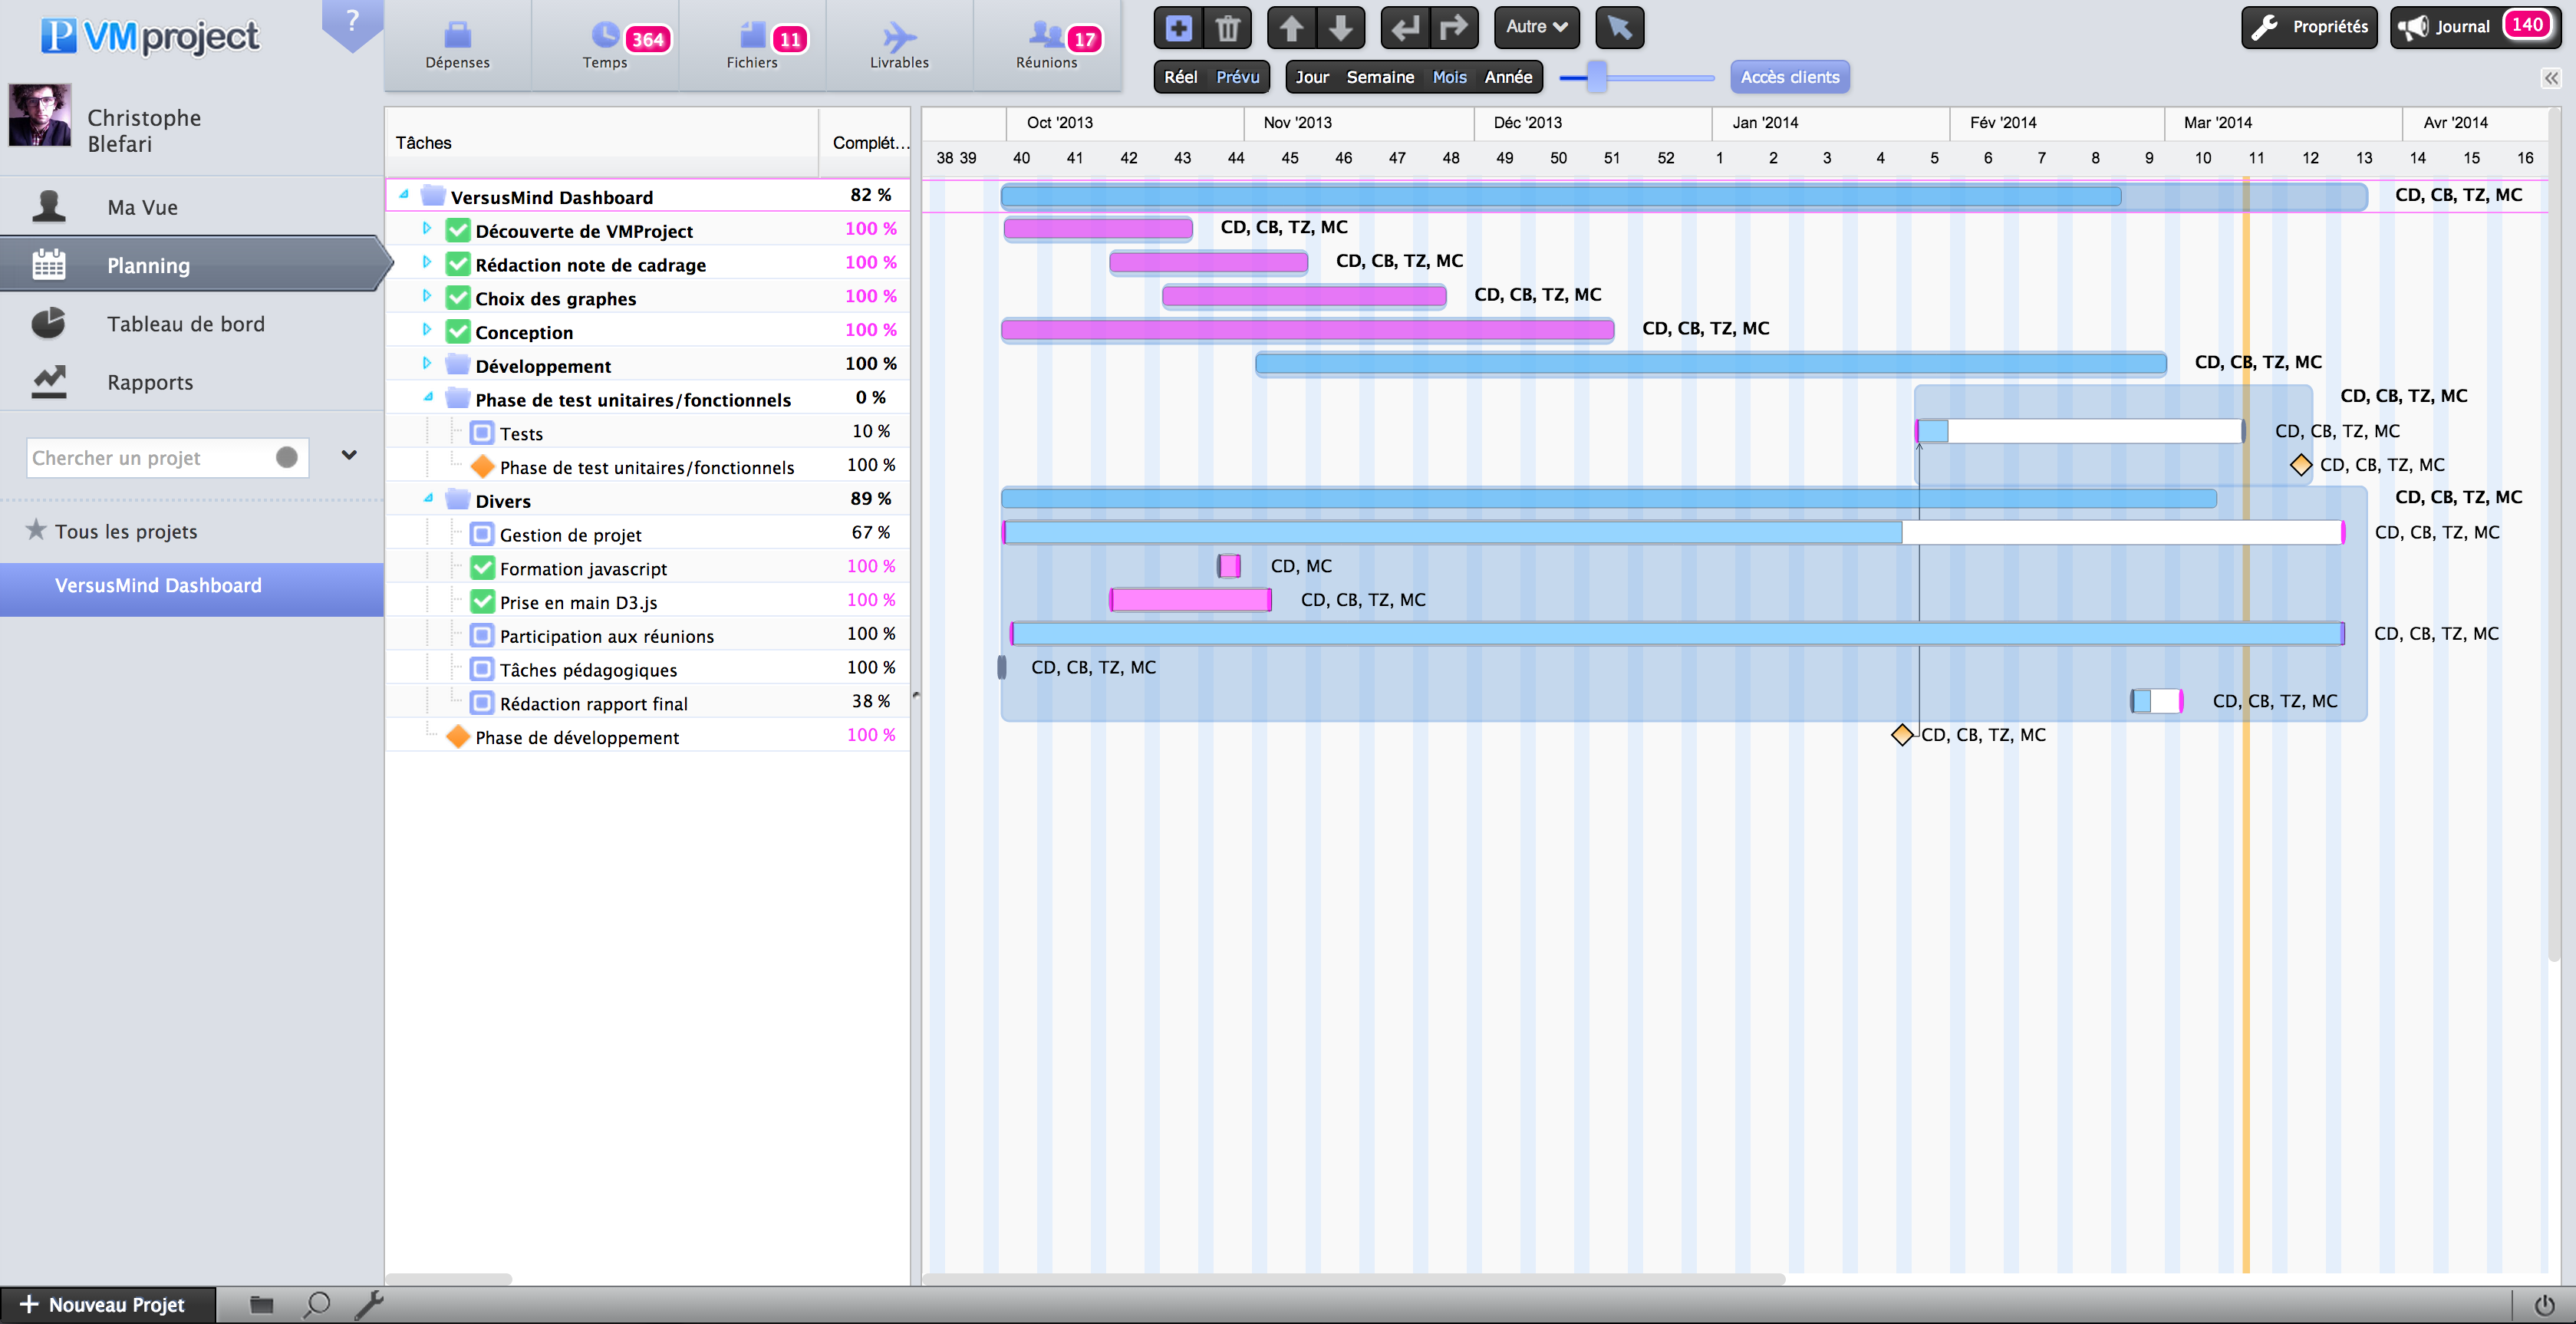
\includegraphics[width=1\textwidth]{pictures/exemple_planning_previsionnel.png}
	\caption{Exemple de planning prévisionnel sur VMProject}
	\label{1}
\end{figure}

Le planning prévisionnel est coloré selon l’avancement, la ligne jaune verticale représentant le jour actuel.\\

Les onglets sur la gauches sont les menus principaux, à savoir que \textbf{Ma vue} correspond à la partie propre à chaque utilisateur, la partie \textbf{Tableau de bord} correspond à l’endroit où devra apparaître notre projet, et la partie \textbf{Rapports} affiche, comme indiqué ci-dessous figures \ref{2} et \ref{3}, un bilan d’activité sur le projet.\\

\begin{figure}[H]
	\centering
	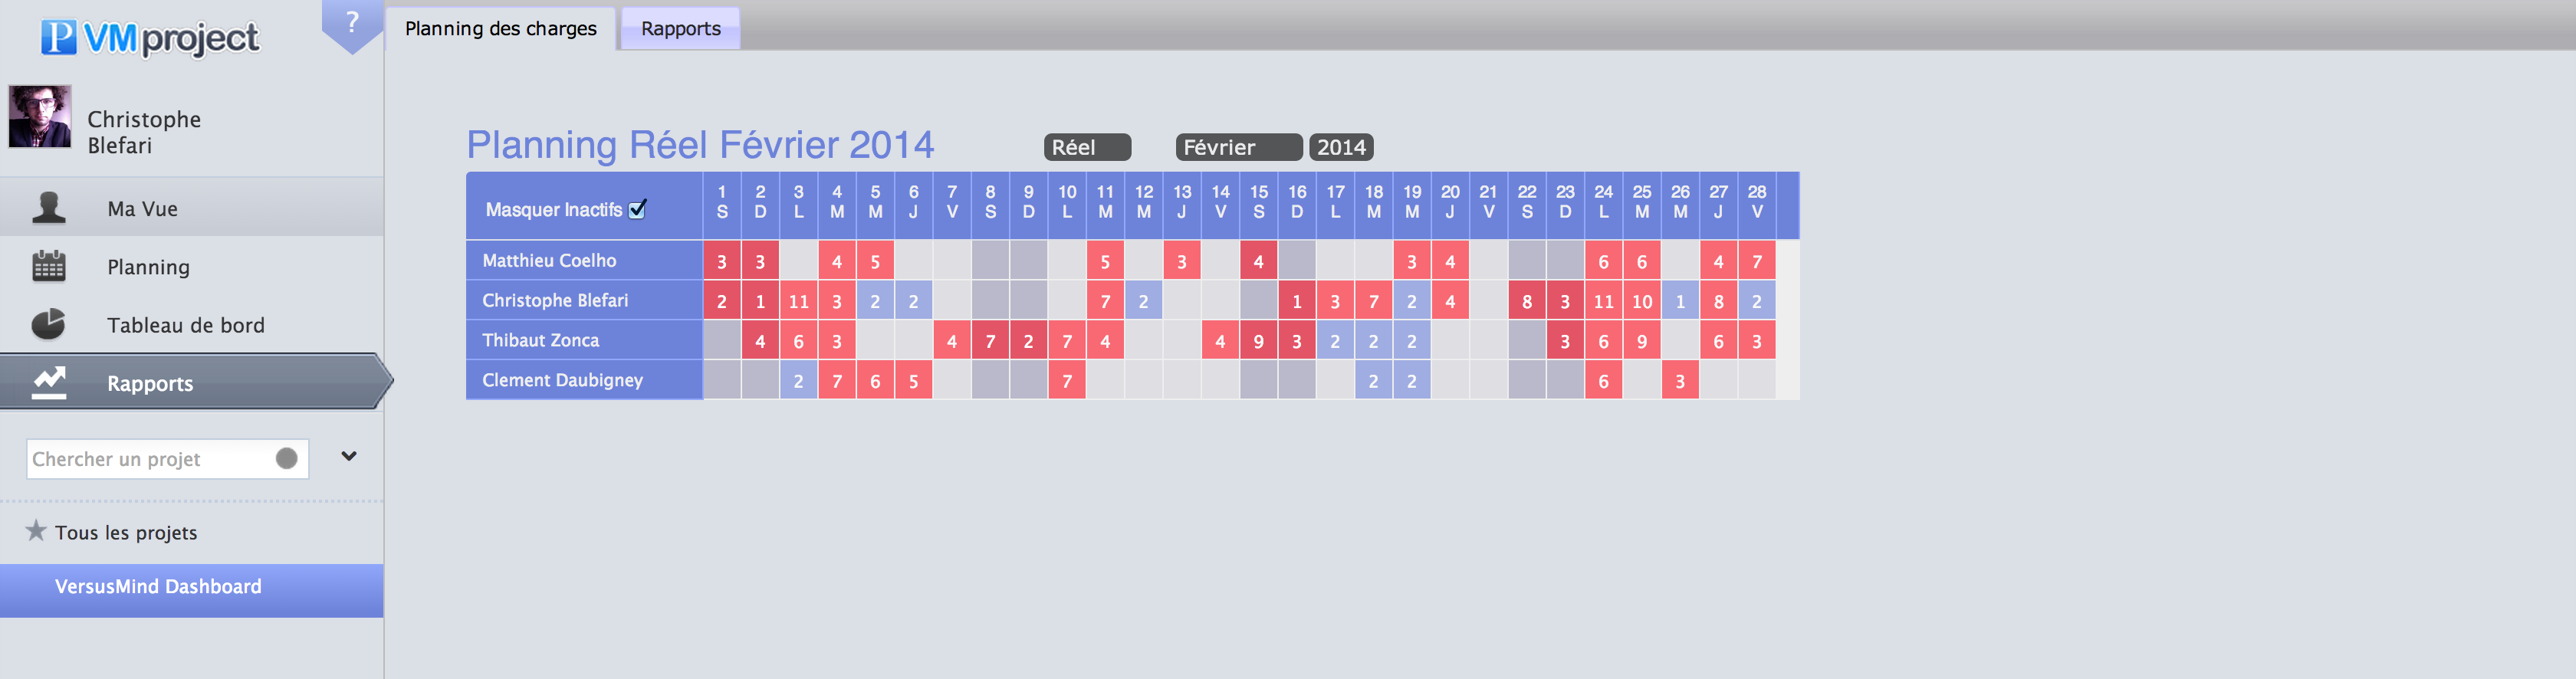
\includegraphics[width=1\textwidth]{pictures/rapport1.png}
	\caption{Rapport, planning des charges}
	\label{2}
\end{figure}

Nous pouvons aussi générer un rapport horaire global ou pour chaque utilisateur. On retrouve donc le nombre total d’heures passées sur un projet ou tous les projets, ainsi que la répartition du nombre d’heures passées sur les différentes tâches.

\begin{figure}[H]
	\centering
	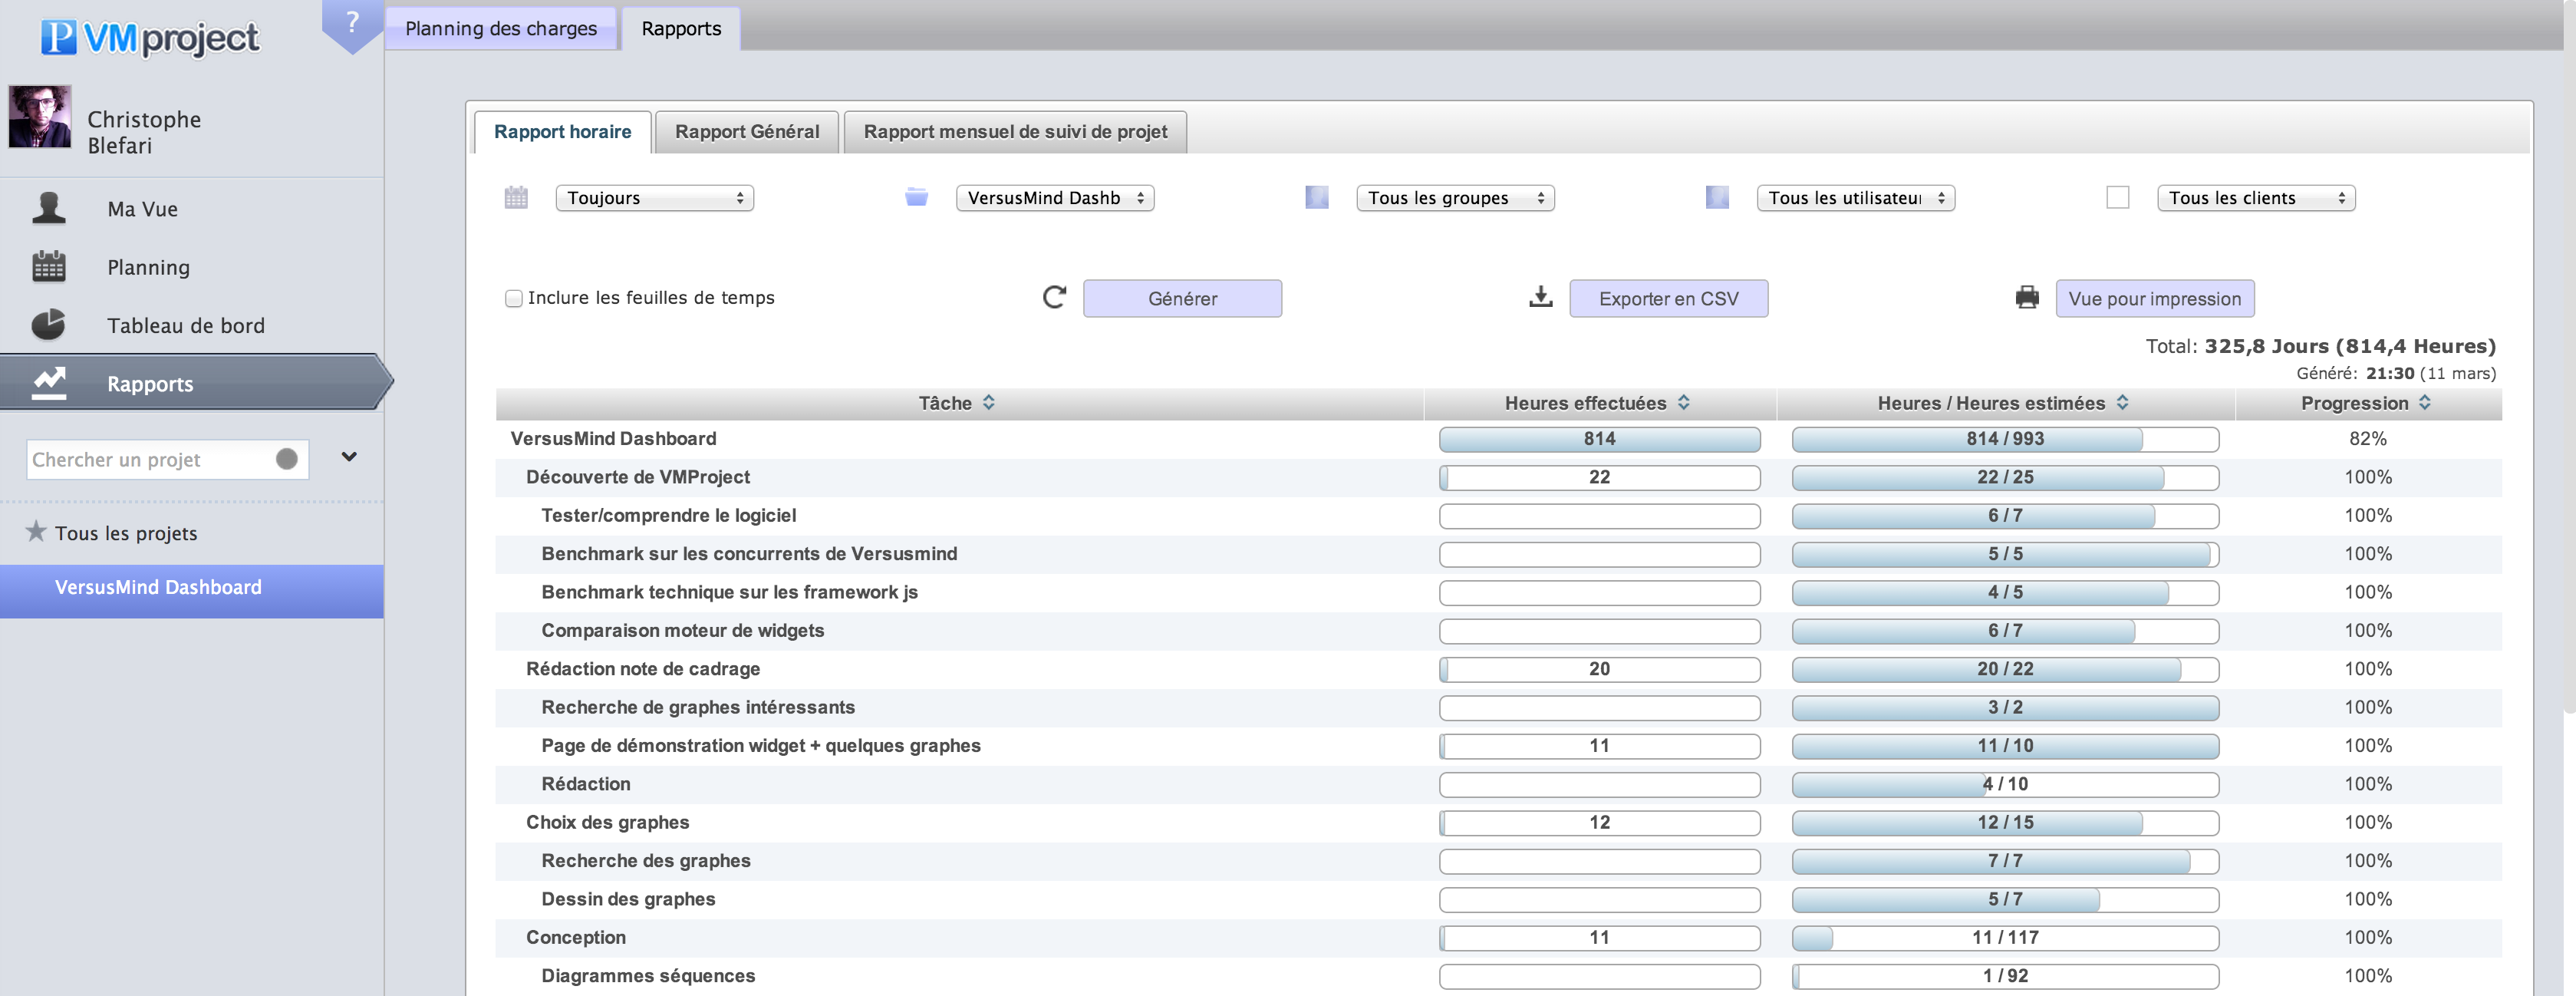
\includegraphics[width=1\textwidth]{pictures/rapport2.png}
	\caption{Rapport, calcul des rapports en fonction des différentes données}
	\label{3}
\end{figure}


\chapter{Notre projet : réalisation d'une dashboard}
  
  \section{Définition d'une dashboard}
  
Dashboard signifie tableau de bord en français. La définition de dashboard donnée par Peter McFadden est la suivante : \emph{Une interface utilisateur en temps réel, facile à lire, souvent d’une seule page, montrant une représentation graphique de l'état actuel (instantané) et les tendances historiques des principaux indicateurs de performance d'une organisation pour permettre des décisions instantanées en un coup d'œil}. Ce terme provient de l’industrie automobile. Dans une voiture, le tableau de bord affiche la vitesse, l’essence, le compte-tour… Soit toutes les informations essentielles à la bonne conduite, et ce rapidement, en un coup d’œil. L’objectif est le même en terme de gestion de projet : le chef de projet a besoin de connaitre rapidement les informations essentielles et pertinentes de son projet. Ces informations sont les critères principaux du projet comme le budget, les ressources, le temps restant, le retard… \\

Cependant, ces critères restent à déterminer. Au final, une dashboard est un aperçu lisible et rapide des données essentielles d’un projet. Il apparait rapidement que le meilleur moyen de réaliser cela est l’utilisation de graphes : une grande quantité d’informations peut être rapidement représentée. Comme le montre l’exemple de la dashboard de Squiz Analytics (fig. \ref{a1}), quelques graphes harmonisés par un jeu de couleurs explicites rend aisée la lecture. L’exemple d’iGoogle (fig. \ref{a2}) reprend cet aspect d’affichage graphique en y ajoutant un partitionnement des données afin de structurer la page et surtout d’adapter le type de représentation au critère affiché ; en effet, il apparait incohérent de représenter le budget sur une courbe, un graphe en camembert semblant plus adapté. Une fois les critères sélectionnés, il est donc important de trouver la méthode de représentation la plus adaptée, à savoir que la plus compliquée est souvent loin d’être la meilleure ; certaines données sont d’autant plus parlante avec une simple donnée chiffrée.
  
  
  \section{Existant sur VMProject}
  
  Un tableau de bord existe déjà sur VMProject. Il présente différents graphes (10 au total) représentant divers critères plus ou moins pertinents tels que les charges restantes, l’avancement, les charges par ressource par semaine… comme le montre la figure \ref{4}.\\
  
\begin{figure}[H]
	\centering
	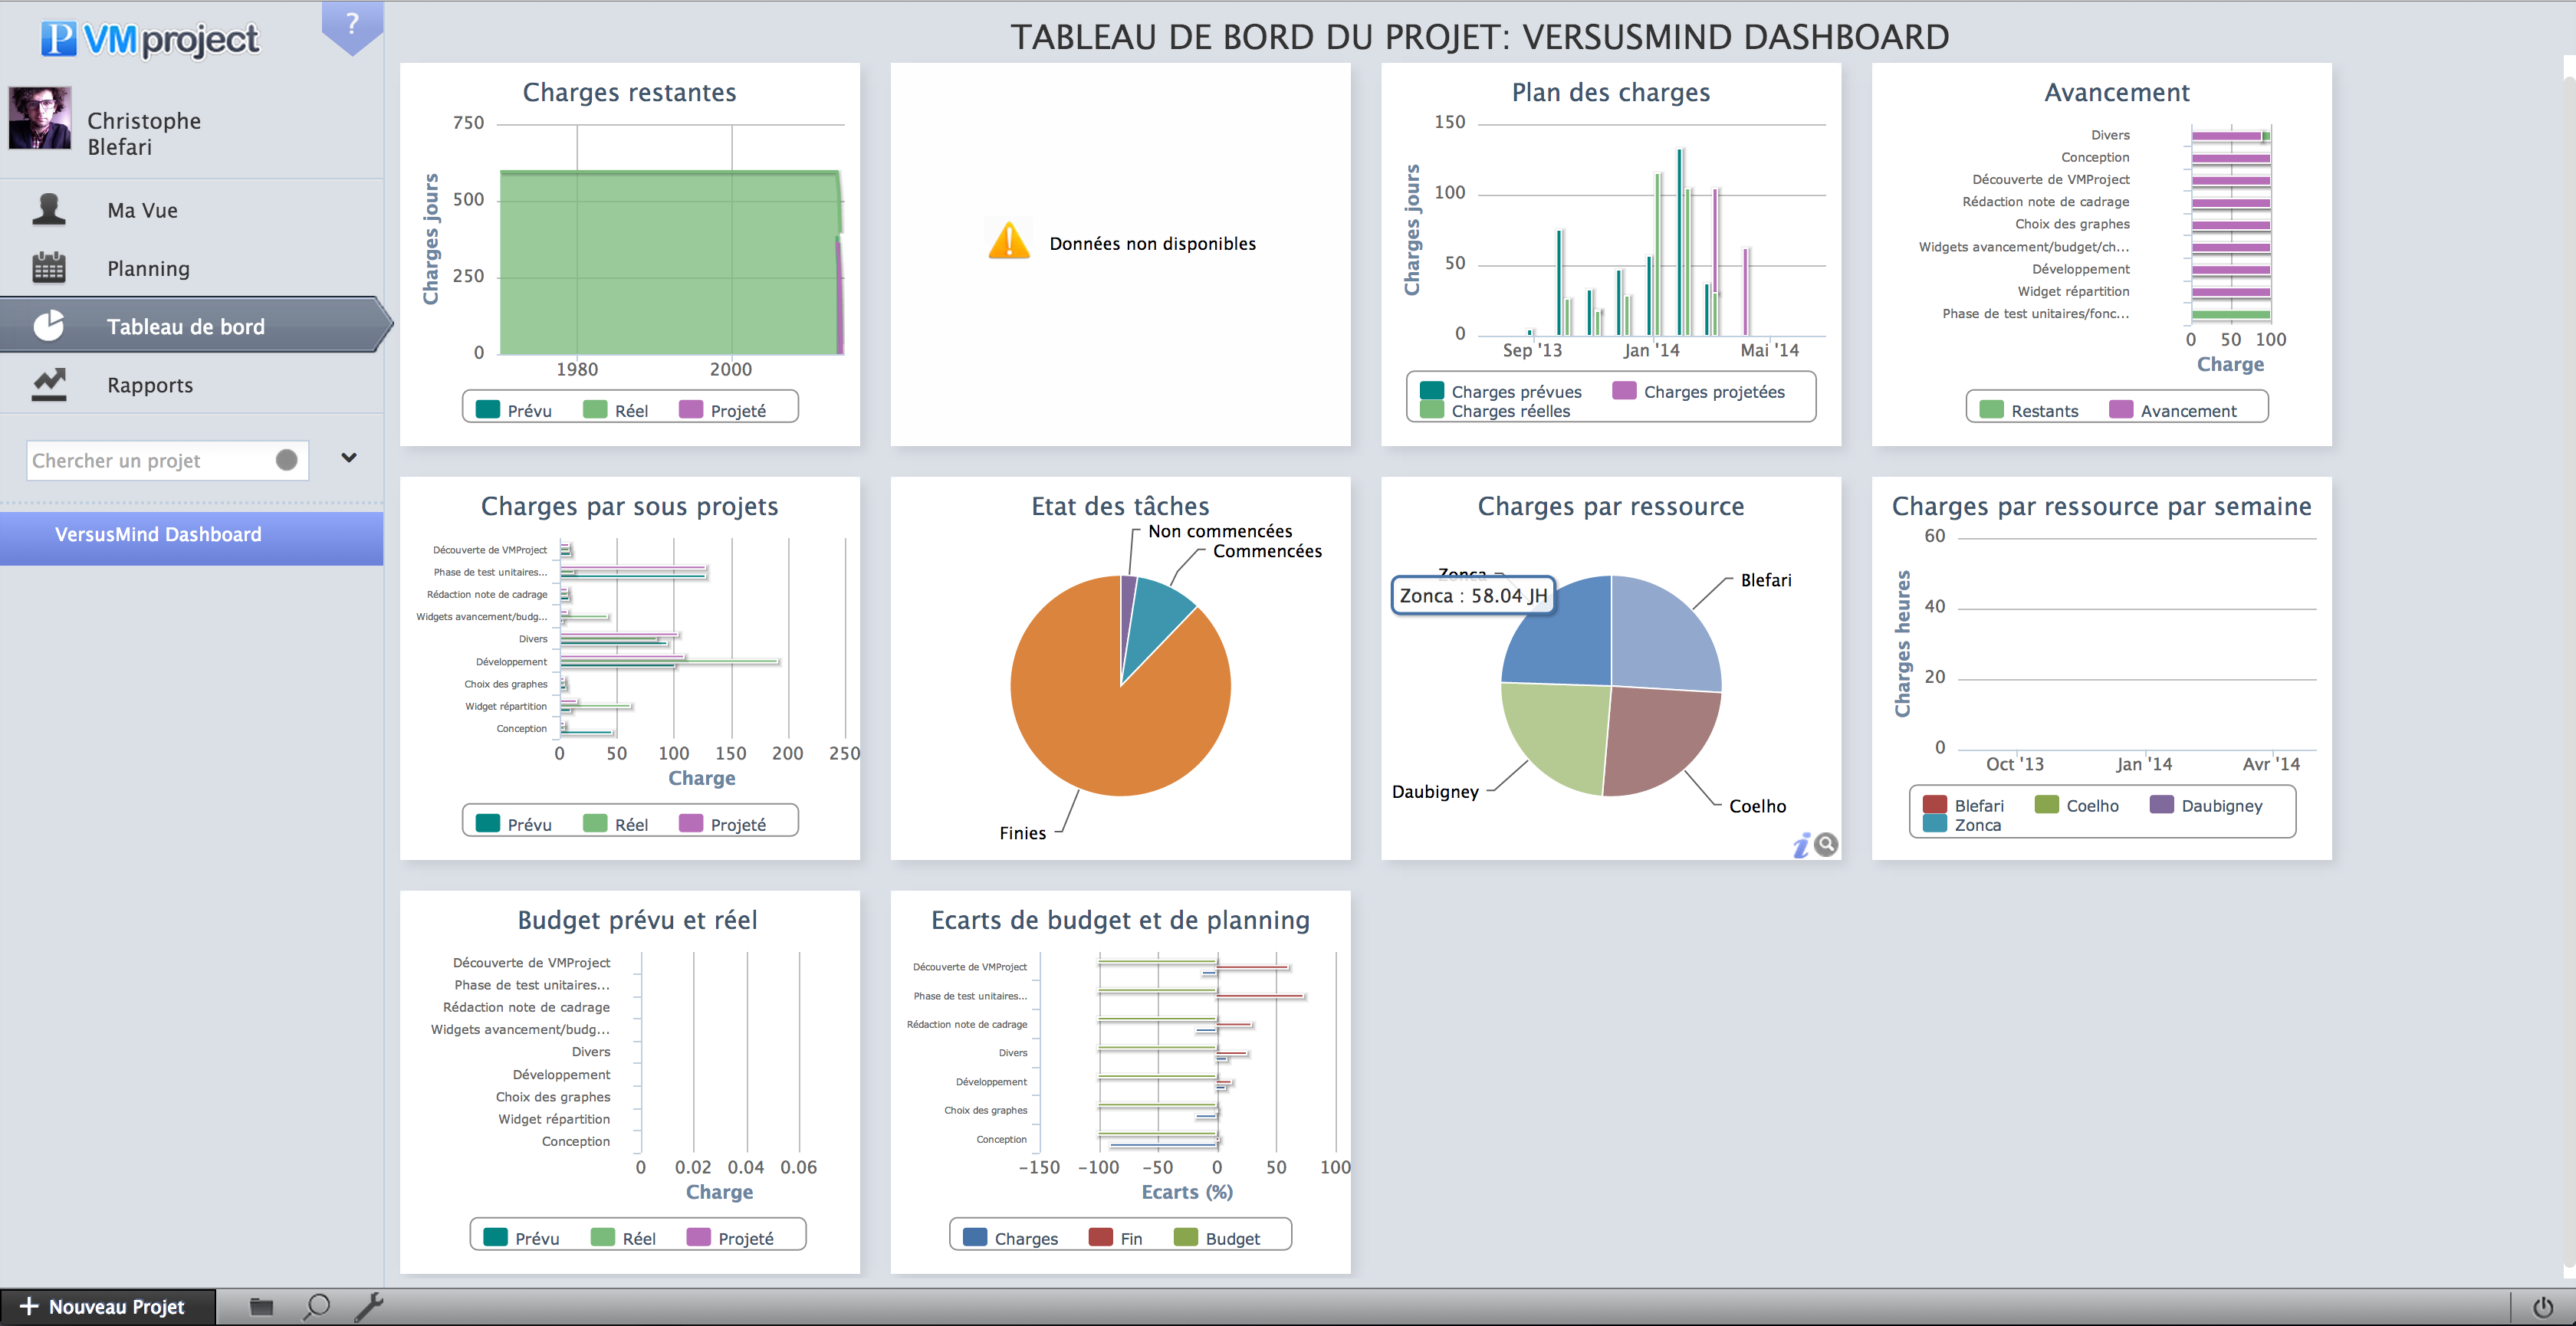
\includegraphics[width=1\textwidth]{pictures/dashboardexistant.png}
	\caption{Dashboard existante sur VMProject}
	\label{4}
\end{figure}
  
  
  Cependant, plusieurs critiques peuvent être émises à propos de cette dashboard et de son efficacité. En effet, il apparait relativement compliqué de connaître rapidement toutes les données importantes du projet concerné. Les graphiques sont un moyen efficace pour afficher les informations, mais non-exhaustif ; il convient d’y joindre des données plus brutes comme des chiffres simples ou des commentaires, d’autant plus qu’un graphe seul présente parfois peu d’intérêt sans explication. Ici, il y a beaucoup de graphes, donc l’information recherchée est plus dure à trouver. Ce nombre important rend chaque graphique petit pour s’adapter à la taille de la page et donc illisible. Un grossissement est nécessaire à chaque fois, ce qui n’est pas optimal en temps. D’autant plus que la miniature des graphiques présentés n’est parfois pas cohérente avec le graphe en taille réelle ; prenons l’exemple des charges par ressource par semaine. La miniature présentée sur la figure précédente laisse croire à un graphe vide, sans données. Or le grossissement prouve le contraire, comme on peut le voir sur la figure \ref{c1} : 

\begin{figure}[H]
	\centering
	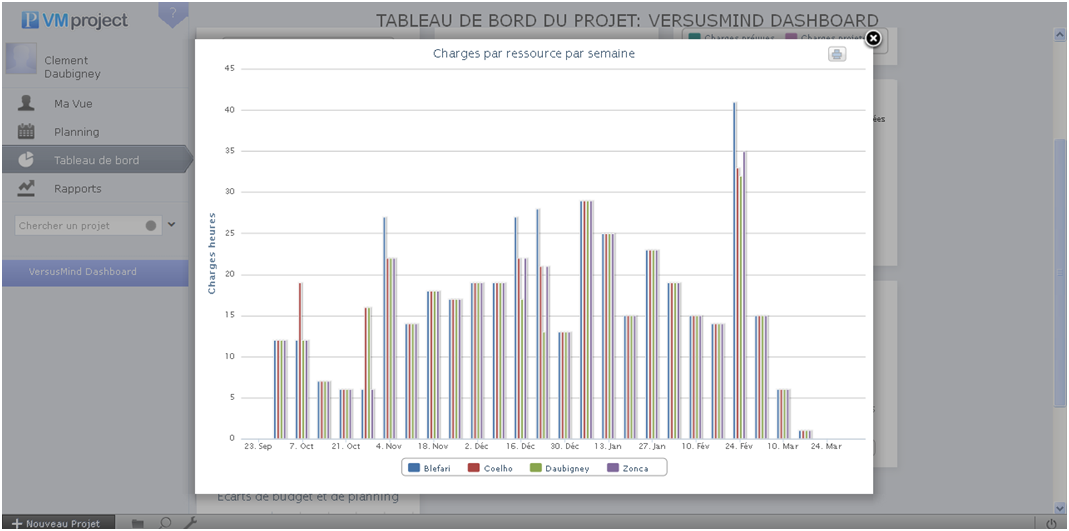
\includegraphics[width=1\textwidth]{pictures/clement/c1.png}
	\caption{Existant, présentation des charges par ressources/semaine}
	\label{c1}
\end{figure}
  
  Mais la place allouée au graphique par rapport aux informations qu’il présente est bien trop petite ; on perd ici tout l’intérêt de la dashboard. D’une part, le graphe est présenté mais doit être grossi pour être lu, donc la notion de rapidité est perdue, et d’autre part, ce graphe ne fournit aucune donnée ce qui peut même être considéré comme une information contradictoire lorsque seule la miniature est affichée. Ici, c’est la notion de lisibilité qui est mise en défaut.
Les données sont peu claires, peu précises (certains graphes ne s’affichent parfois pas), et le design de la page est assez simpliste. Les différents graphiques sont malgré tout cliquables en partie. Cela permet de restreindre les données affichées à une seule ressource ou à un seul aspect (réel – prévu – projeté) selon le graphe, et à obtenir un peu de détail sur les camemberts. Toutefois, on ne peut pas obtenir le détail des en fonction des tâches ; les données sont affichées pour le projet en entier. \\
  
Enfin, la pertinence des données est contestable : le graphique Etat des tâches n’apporte pas beaucoup d’informations. Savoir qu’un tel nombre de tâches est terminé ne donne pas nécessairement d’indications sur l’avancement du projet étant donné que chaque tâche peut avoir des durées et des importances différentes. De même, le graphe Charges par ressources par semaine montre ses limites dans le cadre d’un projet de grande envergure et surtout de longue durée, ne donnant aucune flexibilité au niveau de la plage d’affichage. Avec le nombre de semaines grandissant, les données vont devenir illisibles et futiles.\\
  
  \section{Objectifs et périmètres du projet}
  
Notre projet consiste donc concrètement à créer une nouvelle page qui permettra aux chefs de projet de rendre la gestion beaucoup plus synthétique et aisée. Nous devons donc partir de zéro pour concevoir la nouvelle dashboard de VMProject. Comme décrit dans la note de cadrage, VersusMind est le maître d’ouvrage et nous, étudiants de TELECOM Nancy, sommes les maîtres d’œuvre.\\
L’objectif est donc de créer un nouveau tableau de bord pour VMProject intégrant plusieurs fonctionnalités. Il nous faudra dans un premier temps déterminer les données à afficher sur cette page (certaines informations sont plus pertinentes que d’autres), selon ce que proposent les clients, tout comme les concurrents sur leurs propres solutions.\\
Il est donc nécessaire d’effectuer un tour d’horizon des concurrents et une sélection du support technique le plus adapté. Il est primordial de définir clairement les étapes du projet avant de commencer le développement, pour éviter toute perte de temps. S’en suivra ensuite une phase de tests afin d’assurer la qualité du produit fini.\\
Au niveau du produit en lui-même, les objectifs sont :\\
\begin{itemize}
\item Une interface moderne
\item L’affichage des graphiques doit être rapide
\item La disposition des graphiques sur la page doit être modifiable
\item Offrir une interaction avec le client en lui donnant la possibilité de choisir lui-même les informations à afficher.\\
\end{itemize}
Initialement, nous nous étions mis d’accord avec notre maitre d’ouvrage pour concevoir un outil simple d’utilisation, clair et compréhensible par tous. C’est en effet l’un des buts premiers d’un tableau de bord : la lisibilité et la simplicité. VMProject était alors un produit utilisable par tous, quel que soit le niveau de formation et les connaissances en gestion de projet ; ce logiciel était d’ailleurs gratuit le premier mois pour un test en production.\\
Or pendant notre projet, la ligne de conduite de VersusMind sur certains points a changé, influençant directement les objectifs de notre travail. L’entreprise nancéenne  a choisi de professionnaliser et d’expertiser l’accès à VMProject ; en ne proposant plus que des démonstrations sur rendez-vous et en ne permettant l’utilisation directe qu’aux souscripteurs, VersusMind pense limiter l’accès à la future dashboard uniquement aux connaisseurs de la gestion de projet. C’est pourquoi il nous a été demandé à cet instant d’orienter notre conception sur des graphes contenant plus d’informations donc également plus complexes à comprendre. \\
Le projet sera documenté, le code commenté, et des réunions régulières sont tenues avec nos encadrants universitaire à TELECOM Nancy, de même qu’avec les encadrants industriels.\\

\chapter{Méthodes de travail}

	\section{Gestion de projet}
		\subsection{Gestion humaine}
		
En informatique il est nécessaire de faire de la gestion de projet. En effet tous les projets doivent être gérés par un chef de projet qui centralise les informations et les communications avec les acteurs extérieurs. Le chef de projet doit avoir une vision d’ensemble sur le projet tout en sachant quel sont les forces et les faiblesses de chacun pour permettre à ses ressources de travailler le plus efficacement possible. C’est pourquoi dans ce travail pédagogique il nous a été tout d’abord demandé de créer une équipe autour d’un chef de projet. Nous avons défini Christophe Blefari comme chef de projet. Ainsi la tâche qui est sienne est en premier lieu de planifier les réunions avec l’entreprise VersusMind, mais aussi avec nos encadrantes universitaires. De plus il doit réaliser le planning prévisionnel et attribuer les tâches aux collaborateurs : Matthieu Coelho, Clément Daubigney et Thibaut Zonca.\\

%photo de l'équipe

Ensuite, l’entreprise a mis à notre disposition un encadrement de qualité. Nous avons été supervisés par Monsieur Benoît Zohar qui est le chef technique de VersusMind, mais aussi par Monsieur Maxime Riggi — un ancien étudiant de l’ESIAL. Ils ont essayés donc d’être au maximum présent tous les deux à nos réunions pour que cela augmente les échanges et la réflexion sur le produit. De plus Monsieur Benoît Koch, qui est le directeur de l’entreprise, a assisté très régulièrement à nos réunions pour connaître l’avancée du projet. Et vers la fin la nouvelle directrice de produit de VMProject Mme. Julie Pavillon a aussi assisté à nos réunions pour être au courant sur notre projet. On remarquera que nous avons eu beaucoup d'interlocuteurs sur le projet. Cela a été un avantage mais aussi un désavantage car si les réflexions et les idées pouvaient murir plus vite, beaucoup de décisions se sont rendues plus floues par la présence de ces multiples sources de communications. Pour tenir les comptes nous nous sommes réunis avec l’entreprise à quinze reprises au cours du projet.\\

Du côté universitaire, nous avons été encadrés par Madame Marie-Noelle Flavenot et Madame Marie-Claire Cesare qui sont deux enseignantes de l’école dans le domaine du management et de la gestion de projet. C’est pourquoi leurs conseils sur le projet se sont avérés précieux et nous ont aidé à avoir une vision plus claire sur nos objectifs et sur le travail à réaliser. Au cours des réunions et soutenances blanches avec elles nous avons beaucoup échangé et appris sur la gestion de projet et surtout sur les points de reflexions nous permettant de nous améliorer. Nous avons au final tenu cinq réunions avec elles.\\

		
		\subsection{VMProject}
		
		\begin{figure}[!h]
	\centering
	
\includegraphics[width=0.4\textwidth]{pictures/vmplogo.png}
\end{figure}
		
		
Ainsi, après avoir désigné le chef de projet, il nous a été aussi imposé de travailler avec le logiciel de gestion de projet pour lequel nous développons une fonctionnalité : VMProject. Cela a été pour nous un avantage car nous avons dû passer du temps à comprendre la complexité de l’application, et nous pouvons maintenant l’utiliser comme une équipe l’utiliserai dans une entreprise. Aussi, le planning prévisionnel a été spécifié dans l’application, les réunions ont été ajoutées avec leur compte-rendu et les feuilles de temps sont ajoutées au fur et à mesure de l’avancement du projet.\\

Les feuilles de temps sont l’élément clé de notre gestion de projet. Le projet étant à but industriel mais via un cadre pédagogique, il faut donc que les acteurs du projet puisse retracer le temps que nous y avons consacré. VMProject propose  donc une fonctionnalité qui permet aux développeurs d’ajouter une feuille de temps avec une durée, une date et une justification dès qu’un travail sur une tâche est effectué. Par la suite l’application va calculer l’avancement qu’a apporté l’ajout de cette feuille de temps. C’est ainsi que notre gestion de projet est réalisée. Nous pouvons maintenant voir l’avancement de toutes nos tâches en un clin d’oeil en allant dans l’application VMProject.\\

		\subsection{Outils et git}
		
\begin{figure}[!h]
	\centering
	
\includegraphics[width=0.4\textwidth]{pictures/gitlogo.png}
\end{figure}
		
Pour finir sur la gestion de projet, nous utilisons aussi git pour le versionage et le partage du code source. À l’heure actuelle git est un outil incontournable dans tous les projets web car il permet de versioner le code et de travailler à plusieurs sur un même fichier sans faire face à de conflits trop importants, grâce à sa structure de données purement fonctionnelle.\\

Ainsi matériellement notre structure de travail est très simple. Nous développons sur nos machines personnelles en ayant accès au code source complet de VMProject, puis dès qu’une modification ou une fonctionnalité est prête à être partagée nous la poussons — git push — sur le serveur git privé de la société. De plus nous avons à notre disposition un serveur de développement sur lequel nous synchronisons nos fichiers locaux pour le développement, l’application étant trop lourde et trop complexe nous ne pouvons pas la lancer sur nos ordinateurs personnels.\\

Après pas mal de temps nous nous sommes rendus compte qu'il était judicieux de créer une conversation Skype nous incluant tous pour permettre des échanges plus rapides sur le projet. C'est pourquoi nous avons donc commencé à travailler des cette manière en se réunissant sur Skype pour discuter et avancer sur le projet. En particulier pour mettre des verrous sur le serveur et éviter des conflits de développement.\\

De plus nous avons créé une mailing list pour n'oublier personne lors de la communication avec VersusMind.

Nous avons donc vu ce qui concerne la gestion de notre projet en terme de ressources matérielles et technologiques, mais aussi en terme de ressources humaines.\\

	\section{Planning previsionnel}
	
	Voici le planning prévisionnel que nous avons mis en place au début du projet :\\

\begin{itemize}
\item \emph{Découverte de VMProject (30/09/2013 - 22/10/2013)} : 

Le but de cette première étape primordiale est tout simplement de se familiariser avec l'outil de gestion de projet qu'est VMProject, en utilisant toutes les fonctionnalités proposées par l'application.\\

\item \emph{Rédaction des spécifications (23/10/2013 - 06/11/2013)} :

Dans un premier temps, il faudra rechercher les informations à mettre en avant dans le tableau de bord. Puis chercher quels outils techniques qui seront le mieux adaptés au besoin du client pour ce projet en particulier.\\

\item \emph{Sélection des types de graphiques (07/11/2013 - 24/11/2013)} :

Ensuite il faudra sélectionner différents graphiques, les plus pertinents possibles, afin de représenter au mieux les données dont nous disposerons.\\

\item \emph{Création d'une maquette de notre tableau de bord (25/11/2013 - 02/12/2013)} :

Une fois que les principaux choix de conception sont faits, il est bon de créer une maquette donnant une image du rendu du développement futur. C'est ce que nous ferons au cours de cette étape.\\

\item \emph{Phase de développement (03/12/2013 - 26/01/2014)} :

C'est la phase de développement qui sollicitera le plus les membres de notre équipe. Au cours de cette partie, nous développerons tout ce qui aura été décidé auparavant. Les principaux éléments seront répartis entre les collaborateurs pour travailler de manière efficiente.\\

\item \emph{Phase de test (27/01/2014 - 17/03/2014)} :

Enfin la dernière étape, qui est avec celle de développement une des plus longues. La phase de test permet de déceler tous les bugs de notre travail. C'est aussi le moment de tester le tableau de bord avec des "vraies" données de projets réels, ce qui dévoile souvent des problèmes supplémentaires.\\

\end{itemize}

	\section{Planning réel}

Après avoir vous avoir décrit le planning prévisionnel, nous allons désormais présenter notre planning réel. Bien sûr, des différences apparaissent car nous ne pouvions pas prévoir tout le déroulement du projet à l'avance.\\

Dans un souci de cohérence nous allons vous présenter le planning réel de notre travail sur le projet pour vous permettre de comparer avec facilité avec la planning prévisionnel présenté dans la section précédente. De plus la logique de notre rapport dans la suite est telle qu’elle présente d’une manière logique en premier lieu la phase de conception et ses choix technologiques qui ont entrainés la phase de développement dans son ensemble.\\

\begin{itemize}

\item \emph{Découverte de VMProject (05/10/2013 - 14/10/2013)} :

Dans cette étape, nous avons testé VMProject sous toutes ses coutures. Nous avons créé notre propre instance de VMProject afin de pouvoir ajouter des collaborateurs, des tâches ainsi que d’autres paramètres, pour pouvoir nous familiariser avec l’outil. Nous avons aussi pu faire un tour des concurrents directs de l'application. Bien entendu, cette tâche est indispensable avant de commencer quoi que ce soit d’autre sur le projet.\\

\item \emph{Rédaction des spécifications (14/10/2013 - 02/11/2013)} :

Au cours de cette étape, nous avons recherché les points importants que devait présenter notre dashboard. Nous avons réfléchi aux outils techniques dont nous aurons besoin, tels que la librairie D3.js ou encore le moteur de widget Gridster, un plugin de jQuery.\\

\item \emph{Sélection des types de graphiques (02/11/2013 - /11/2013)} :

Cette étape, avec la rédaction des spécifications, était sans doute la plus difficile. Une fois que nous savions comment nous allions présenter les données au sein de notre tableau de bord, nous avons dû imaginer ce qu’un chef de projet doit voir pour savoir comment son projet évolue. Après de nombreuses recherches, nous avons réussi à nous mettre d’accord avec VersusMind pour ne garder qu’un certain nombre de graphiques sur notre dashboard.\\

\item \emph{Création d’une maquette de notre tableau de bord (24/11/2013 - 06/12/2013)} :

Les choix de conception ayant été faits, nous avons continué notre travail en créant une maquette de notre dashboard, à l’aide de Photoshop. Une fois celle-ci terminée, nous l’avons transmise à l’ergonome et graphiste de VersusMind, qui nous a rendu une version plus en accord avec le futur thème de VMProject, mais aussi plus complexe. Cette maquette allait alors correspondre à ce que nous allions développer.\\

\item \emph{Phase de développement (07/12/2013 - 10/03/2014)} :

Nous avons enfin pu commencer le développement au cours du mois de Décembre. Les premières semaines du mois, nous nous sommes d’abord familiarisés avec le code de VMProject, afin d’en comprendre les détails de fonctionnement. Ensuite, nous avons pu commencer le développement des éléments de la maquette qui nous avait été envoyés plus tôt.\\

\item \emph{Phase de test (20/01/2014 - 17/03/2014)} :

Plutôt que d'attendre la fin de la phase de développement, nous avons commencé à tester nos divers éléments dès que ceux-ci furent terminés. Cette phase s'est intensifiée à partir de la moitié du mois de Février, lorsque les dernières principales fonctionnalités ont été apportées.\\
\end{itemize}

	\subsection{Conclusion sur la gestion de projet}
	
	Nous avons appris à nos dépends que la gestion de projet n'était pas un exercice facile, en effet réaliser un planning prévisionnel est une tâche ardue car nous ne pouvons jamais prévoir tout à l'avance. Comme nous pouvons le voir avec les plannings présentés précédemment, les périodes n'ont pas été respectées. Mais cela nous a montré la difficulté de gérer un projet sur ce point. L'exercice a été très pédagogique.\\
	
	Ensuite la travail en équipe de quatre personnes a été une partie qui nous a énormément appris sur notre capacité à travailler ensemble sur une longue durée. Et en conclusion, nous avons été un groupe plutôt homogène et compatible. Ce qui n'est pas vraiment une découverte, mais une confirmation car nous nous sommes aussi choisi pour notre compatibilité possible.\\
	
	En revanche, sur le plan de la communication avec l'entreprise, nous nous sommes parfois sentis mis à l'écart du processus de décision et des différents objectifs. Mais nous avons aussi appris de cela. Au final nous avons passé environ \textbf{900h} sur le projet.\\

\chapter{Phase de conception}

La phase de conception est une phase essentielle dans la bonne réalisation d’un projet, car elle conditionne tout le déroulement, et influe notamment grandement la phase de développement : si le produit fini recherché est clairement ciblé et clair pour tous, les flottements dans la suite du projet seront moindres. Notre phase de conception a donc plusieurs objectifs successifs : faire un tour d’horizon des concurrents, trouver les critères pertinents à afficher et leur mode d’affichage, et enfin mettre en forme une maquette.\\

	\section{Benchmark des concurrents}

Le tour d’horizon des concurrents de VMProject est la première étape de la conception. C’est en effet le point de départ pour situer le terme de dashboard concernant la gestion de projet. Grâce aux concurrents, nous espérions alimenter notre recherche de critères et éventuellement d’idées pour la mise en forme et l’aspect de notre projet. Une bonne analyse de l’existant concurrentiel est également nécessaire pour comprendre les erreurs à éviter ainsi que les points forts à mettre en avant. A partir d’un listing de VersusMind ainsi que quelques recherches, nous avons étudié onze concurrents, à savoir : Time Performance, Planzone, Atikteam, Freedcamp, 5PM, Atlassian, Genius Inside, Project Plane, SciForma, Project Manager et Plum. Le résultat de notre benchmark se retrouve dans le tableau présenté en Annexe (cf. fig \ref{tabconcu}).\\

La colonne « Dashboard existante et accessible » indique si l’accès à la dashboard pour un test ou même une démonstration est payant, auquel cas nous n’avons pu procéder à l’analyse, et si le concurrent étudié possède une dashboard. Il s’avère malheureusement qu’un certain nombre de concurrents ne laissent pas libre accès à leur dashboard ; en revanche, et malgré le fait que peu d’idées en soient sorties, peu de logiciels de gestion de projet possèdent un réel tableau de bord synthétique et original, ce qui laisse une possibilité d’innovation intéressante et donne une importance non négligeable à notre projet pour le développement de VMProject. Comme indiqué dans le tableau ci-dessus, le concurrent qui nous a le plus inspiré est Time Performance avec son « cockpit », visible sur la figure suivante : \\

\begin{figure}[H]
	\centering
	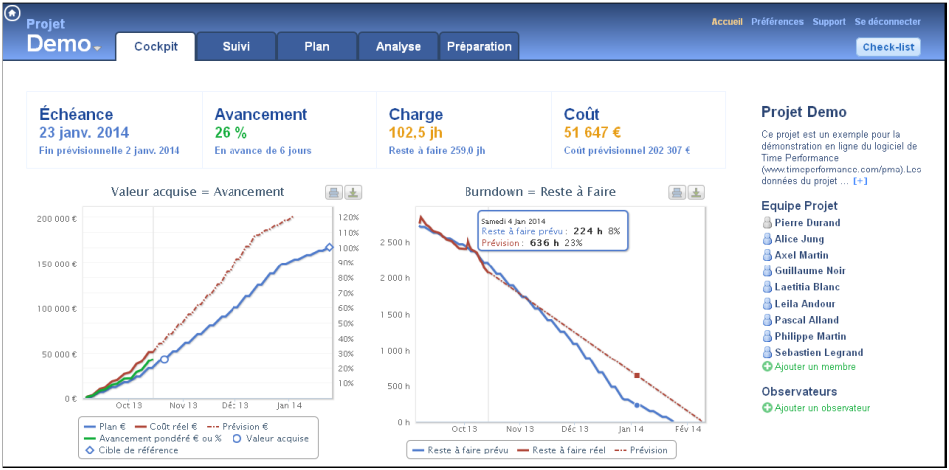
\includegraphics[width=1\textwidth]{pictures/clement/c2.png}
	\caption{Tableau de bord de Time Performance}
	\label{c2}
\end{figure}

Plusieurs points sont pertinents, comme par exemple la liste des membres, l’utilisation de données chiffrées pour l’avancement, la charge et le budget, ou encore l’utilisation de graphes pour symboliser l’avancement. Evidemment, notre projet n’a pas pour but d’effectuer une copie mais une création originale ; c’est pourquoi ce tour d’horizon des concurrents n’est qu’une première étape de la phase de conception mais s’avère néanmoins utile.\\
	
	\section{Étude et recherche de critères pertinents}
	
Nous avons donc ensuite eu a mener une étude et recherche des critères pertinents, étape délicate de ce projet du fait de notre manque d’expérience en terme de gestion de projet. Avec l’aide de nos encadrants universitaires et industriels, nous avons donc établi une liste des critères pertinents :\\

\begin{itemize}
\item Les chiffres clés (avancement, budget…)
\item Un calendrier avec les dates importantes
\item Les écarts de budget
\item La répartition des charges en terme de budget
\item Un burndown chart (graphe représentant le temps de travail restant en fonction du temps)\\
\end{itemize}

Il est important de noter également que VersusMind possède une volonté de conserver trois modes distincts d’affichage des données, à savoir : le mode réel, le mode prévu, et le mode projeté. Le mode réel est bien évidemment ce qu’il s’est réellement produit, et n’est accessible que pour le temps de projet déjà écoulé. Le mode prévu correspond aux données entrées dans VMProject par le chef de projet, au planning prévisionnel en quelque sorte. Le mode projeté est calculé par le logiciel et prend en compte le réel pour faire une estimation du futur. Ces trois différents modes doivent donc apparaître sur la dashboard.\\

	\section{Conception d'une maquette de départ}
	
A partir des critères définis ci-dessus, nous avons pu mettre en forme le moyen d’afficher chaque donnée et concevoir une maquette. Ce travail réalisé grâce au logiciel Photoshop a donné le résultat présenté en fig. \ref{a3}. C'est une maquette simplifiée de notre tableau de bord, composée de plusieurs éléments donnant des informations pertinentes à l'utilisateur sur l'avancement et l'évolution de son/ses projet(s).\\

Nous avons découpé les différentes parties de cette première maquette, de haut en bas et de gauche à droite, pour vous la présenter :\\

\begin{figure}[H]
	\centering
	
\includegraphics[width=1\textwidth]{pictures/notreMaquette/description.jpg}
	\caption{Maquette conception, titre et description du projet}
	\label{5}
\end{figure}


Tout en haut de la page, nous avons prévu un emplacement présentant le titre et la description du projet. Cet élément basique permet de rappeler à l'utilisateur les données qu'il visualise, sous peine de confondre ses statistiques de projets et de les faire échouer suite à des décisions non adaptées.\\

\begin{figure}[H]
	\centering
	
\includegraphics[width=0.7\textwidth]{pictures/notreMaquette/chiffresCle.jpg}
	\caption{Maquette conception, indicateurs}
	\label{6}
\end{figure}

Directement en-dessous, on retrouve des chiffres clés avec des indicateurs colorés permettant de voir l'information recherchée très rapidement. Ces chiffres sont portés sur les données principales que recherche le chef de projet, à savoir le retard, le budget, les charges ou encore la date de fin prévue du projet.\\

\begin{figure}[H]
	\centering
	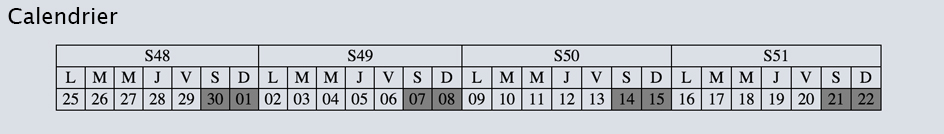
\includegraphics[width=0.7\textwidth]{pictures/notreMaquette/calendrier.jpg}
	\caption{Maquette conception, calendrier}
	\label{7}
\end{figure}

Le calendrier est un élément indispensable de notre tableau de bord. Il affiche les jours, semaines et mois de l'année mais surtout des informations pertinentes comme les réunions,  jalons ou autres livrables prévus dans le temps.\\

\begin{figure}[H]
	\centering
	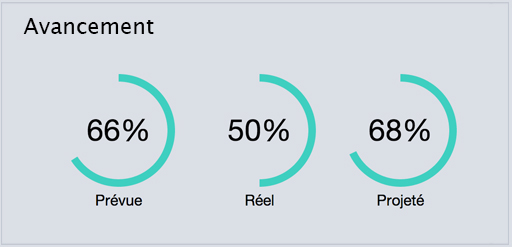
\includegraphics[width=0.4\textwidth]{pictures/notreMaquette/avancement.jpg}
	\caption{Maquette conception, représentation de l'avancement}
	\label{8}
\end{figure}

Voici les premiers graphiques de notre dashboard. Ces trois petits cercles décrivent l'avancement du projet, en mode prévu, réel et projeté. Ces trois modes sont la base de l'application web VMProject, grâce auxquels on peut facilement déduire si le projet est en retard et le temps qui sera nécessaire pour le combler.\\

\begin{figure}[H]
	\centering
	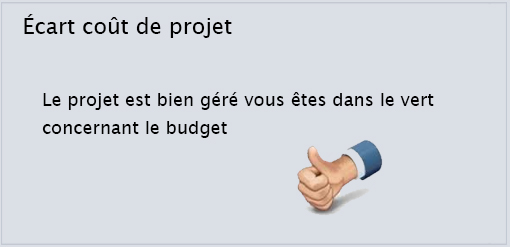
\includegraphics[width=0.4\textwidth]{pictures/notreMaquette/indicateur.jpg}
	\caption{Maquette conception, indicateur sur le coût du projet}
	\label{9}
\end{figure}

Immédiatement à droite des trois petits graphiques que nous venons de présenter, on peut trouver un emplacement dédié à l'écart de coût sur le projet. Le but de cette section est de déterminer grâce aux données de VMProject si le budget est bien géré, et de l'afficher de manière très simple et intelligible pour l'utilisateur final.\\

\begin{figure}[H]
	\centering
	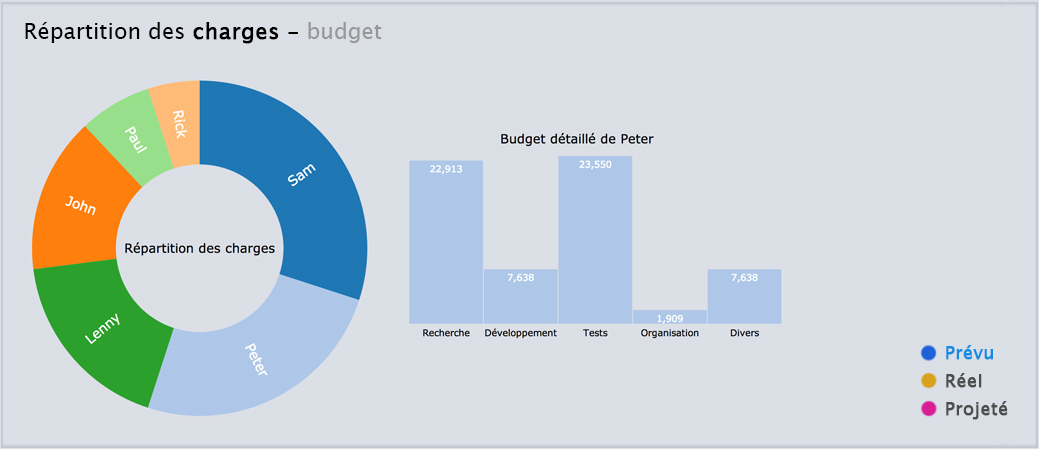
\includegraphics[width=0.6\textwidth]{pictures/notreMaquette/repartition.jpg}
	\caption{Maquette conception, graphe lié de répartition des charges/budget}
	\label{9}
\end{figure}

Plus bas, la page contient un graphique qui présente la répartition des charges et du budget pour les différentes ressources du projet. Ainsi, en cliquant sur un prénom dans le camembert, les données du graphique de droite sont actualisées pour afficher le détail du budget de la personne en question sur les principales phases du projet.\\

En bas de page, nous retrouvons le dernier graphique de notre maquette. C'est un graphique classique de la gestion de projet, qui représente l'avancement du travail de l'équipe par rapport au temps. Il est utile pour voir quand le travail à faire pourra être terminé (cf fig \ref{10}).\\

Enfin, sur la toute droite du tableau de bord, nous retrouvons un panneau (déroulant) présentant les acteurs du projet : les membres de l'équipe et les clients. C'est le dernier élément de notre maquette, qui vient donc compléter notre tableau de bord (cf. fig \ref{11}).\\


Cette maquette n'est certes pas si jolie mais présente tous les points importants que nous pensions intégrer dans notre tableau de bord.

	\section{Maquette finale}

Nous avons donc proposé cette maquette à nos encadrants industriels. La responsable ergonomie de VersusMind a repris nos idées pour l’adapter à la charte graphique de VMProject. Certaines modifications de fond sont également apparues, dues au changement de positionnement de VersusMind par rapport à ses clients suite à la proposition de notre maquette ; initialement, l’entreprise souhaitait quelque chose de simple et compréhensible par tous, puis s’est tournée vers un public plus expert et plus professionnel, à qui on peut se permettre de proposer quelque chose de plus compliqué. La maquette proposée par VersusMind est donnée en fig. \ref{a4}.\\

Comme pour la maquette que nous avions créée, nous allons détailler celle-ci en découpant les éléments un par un. Cela sera particulièrement utile car des modifications importantes et parfois complexes ont été appliquées par rapport à ce que nous imaginions au départ. A nouveau, nous présenterons notre découpage de la maquette de haut en bas, et de bas à gauche.\\

\begin{figure}[H]
	\centering
	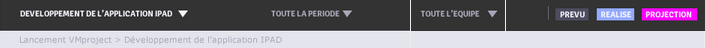
\includegraphics[width=1\textwidth]{pictures/maquetteVersusmind/filtre.jpg}
	\caption{Filtre de notre tableau de bord}
	\label{12}
\end{figure}

Au sommet du tableau de bord, un filtre permet à l'utilisateur de sélectionner une tâche particulière d'un projet, une période donnée ainsi qu'une partie ou la totalité de l'équipe. Toutes les données des graphiques et du tableau de bord en général devront être mis à jour en fonction de ce filtre. 
Sur la droite est située la légende colorimétrique de VMProject pour les modes prévu, réel et projeté. Ces couleurs sont utilisées dans toute l'application et facilite la lecture des données présentées.\\

Cependant, la partie du filtre permettant de choisir des membres ou la totalité de l'équipe sera abandonnée par la suite car ce n'est pas forcément un élément intéressant, étant donné que les graphiques qui suivent comportent déjà ces informations sur les ressources. \\

\begin{figure}[H]
	\centering
	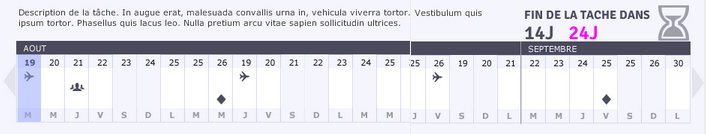
\includegraphics[width=1\textwidth]{pictures/maquetteVersusmind/descriptioncalendrier.jpg}
	\caption{Calendrier et description du projet}
	\label{13}
\end{figure}

Sous le filtre, on retrouve la description du projet ou de la tâche sélectionnée à l'aide du filtre. Le chiffre clé sur la fin du projet s'invite dans cet espace, et cette donnée est désormais affichée en prévu et en projeté (les couleurs bleu foncé et rose correspondent aux modes prévu et projeté, comme nous avons pu le voir dans le filtre).\\
Juste en-dessous, le calendrier a pris des couleurs et des flèches sur les côtés permettent de naviguer dans l'histoire, mais aussi dans le futur du projet. Les réunions, jalons et livrables sont représentés par des icônes livrant leurs détails au survol de la souris.\\

\begin{figure}[H]
	\centering
	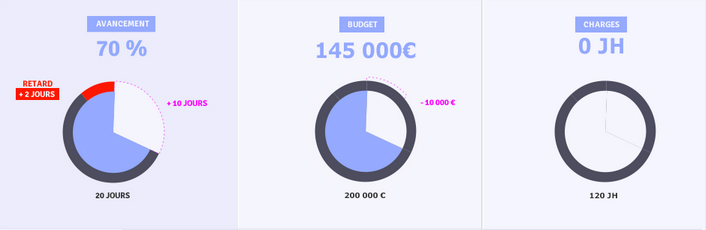
\includegraphics[width=1\textwidth]{pictures/maquetteVersusmind/3graphs.jpg}
	\caption{Graphiques sur les charges, le budget et le retard}
	\label{14}
\end{figure}

Ensuite, nous pouvons remarquer que nos trois petits graphiques ont changés puisqu'ils ont intégré les chiffres clés dont nous parlions, sur le retard, le budget et les charges. C'est une bonne idée puisque les informations portaient sur le même sujet, elles sont désormais rassemblées.\\

A nouveau, il faut se fier au code colorimétrique pour comprendre les graphiques. Le cercle bleu clair correspond au réel, le bleu foncé au prévu et le rose au projeté. Sur le graphique d'avancement, le retard est mis en avant en étant affiché en rouge, pour sauter aux yeux de l'utilisateur.\\

\begin{figure}[H]
	\centering
	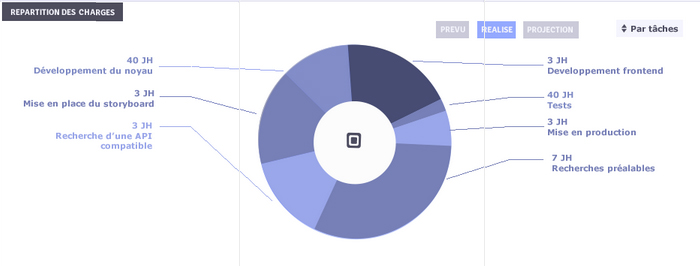
\includegraphics[width=1\textwidth]{pictures/maquetteVersusmind/repartitionInit.jpg}
	\caption{Graphique de répartition dans son état initial}
	\label{12}
\end{figure}

Le graphique suivant étant particulièrement complexe, nous allons expliquer son fonctionnement un peu plus en détail. De base, le tableau de bord affiche un camembert comme sur l'image ci-dessus. Il est possible de changer de mode de données (réel, prévu, projeté) mais aussi de passer du mode "Par tâches" au mode "Par ressources". Il est aussi possible de passer du mode "Charges" au mode "Budget", pour afficher les données en termes de jours-hommes ou de valeur monétaire, mais ce n'est pas affiché sur cette maquette; des sélecteurs à cet effet seront ajoutés en haut à gauche du graphique.\\

De plus, les parts du camembert sont cliquables pour afficher de nouvelles informations, comme sur la figure \ref{15}.\\

Sur le côté de la maquette se situe un petit panneau gris, dépliable avec une flèche, affichant les acteurs du projet : membres de l'équipe et les clients. Ce panneau a peu changé par rapport à notre maquette d'origine et nous ne le détaillerons donc pas plus que cela (cf. fig. \ref{16}).\\


Il faut noter que les éléments principaux, c'est à dire le calendrier et les différents graphiques, sont dans des widgets déplaçables par l'utilisateur, pour lui permettre d'organiser son tableau de bord à sa guise.\\


En définitive, cette maquette nous est revenue plus travaillée, mais surtout bien plus complexe et il nous a fallu un certain temps afin d'en comprendre toutes les subtilités.\\


	\section{Choix techniques}
	
	Pour les choix techniques au sein de notre tableau de bord, nous avons fait les choix suivants. Comme nous l’avons déjà dit plus haut dans ce rapport, nous avons sélectionné la librairie D3.js pour générer et afficher nos graphiques. Cette librairie a pour principaux avantages d’être open-source, d’être très bien documentée et beaucoup utilisée sur internet. De plus, les graphiques sont sobres et peuvent être animés. En Annexe E nous pouvons voir le travail de comparatif que nous avons effectué pour la recherche de cette librairie.\\

Ensuite, VersusMind nous avait transmis leur souhait de pouvoir échanger la position des graphiques entre eux. Pour ce faire, nous avons étudié différentes librairies de widgets.\\

		\subsection{Moteurs de widgets}
		
Afin de rendre le tableau de bord personnalisable, nous devions trouver un moyen pour l’utilisateur de modifier l’emplacement de ces graphiques. Nous avons choisis de mettre chaque élément dans des blocs distincts, appelés widgets. Ils pourront donc par la suite être déplacés pour convenir aux exigences de l’utilisateur.\\

Il existe plusieurs types de programmes permettant de faire ceci, appelés moteurs de widgets. Windows 8 utilise d’ailleurs ce type d’interface pour ses utilisateurs (Interface Métro).\\

Nous devions donc rechercher un outil dont les critères étaient :
\begin{itemize}
	\item Créer différents widgets qu’on peut remplir avec du HTML
	\item Widgets déplaçables
	\item Implémentation possible dans le projet existant
	\item Documentation complète
	\item Gratuit
	\item Libre
	\item Utilisation simple pour l’utilisateur
	\item Compatible avec tous les navigateurs : Internet Explorer 9+, Firefox, Chrome, Safari
\end{itemize}

A partir de plusieurs recherches, nous avons trouvé plusieurs moteurs de widgets qui correspondent à nos critères.
\begin{enumerate}
\item Gridster : \\http://gridster.net/ 
\item Shapeshift : \\http://www.jqueryscript.net/demo/Dynamic-Drag-Drop-Grid-Layout-Plugin-shapeshift/demo/
\item iNETTUTS : \\http://nettuts.s3.amazonaws.com/127\_iNETTUTS/demo/index.html
\item gridly : \\http://ksylvest.github.io/jquery-gridly/
\end{enumerate}
	
	\subsubsection{Mais, lequel choisir ?}
	
	Nous avons établi un tableau comparatif de chaque moteur de widgets. Chaque outil a donc du être testé afin de voir s’il répondait ou non à chacun des critères. Les fonctionnalités de base, à savoir créer des blocs déplaçables, étaient toutes remplies pour chaque moteur, il a donc fallu donner plus de poids à certain critères pour départager ces outils. \\

Le fait d’utiliser un produit documenté permet de l’intégrer beaucoup plus facilement, et donc plus rapidement dans le code source du projet. Ainsi, nous avons essayé d’installer chaque moteur, et nous avons constaté rapidement les différents problèmes.\\
L’intégration était impossible pour cause d’incompatibilité avec la version de jQuery des serveurs de VMProject, ou alors compliquée à cause d’un plugin mal documenté…\\

Il était donc très difficile d’intégrer un moteur de widgets à VMProject. Nous avons finalement choisi d’utiliser Gridster. L’avantage principal de ce plugin jQuery est qu’il est très bien documenté et très utilisé, il bénéficie donc d’une grande communauté et d’une évolution continue.\\
	
	\begin{figure}[H]
	\centering
	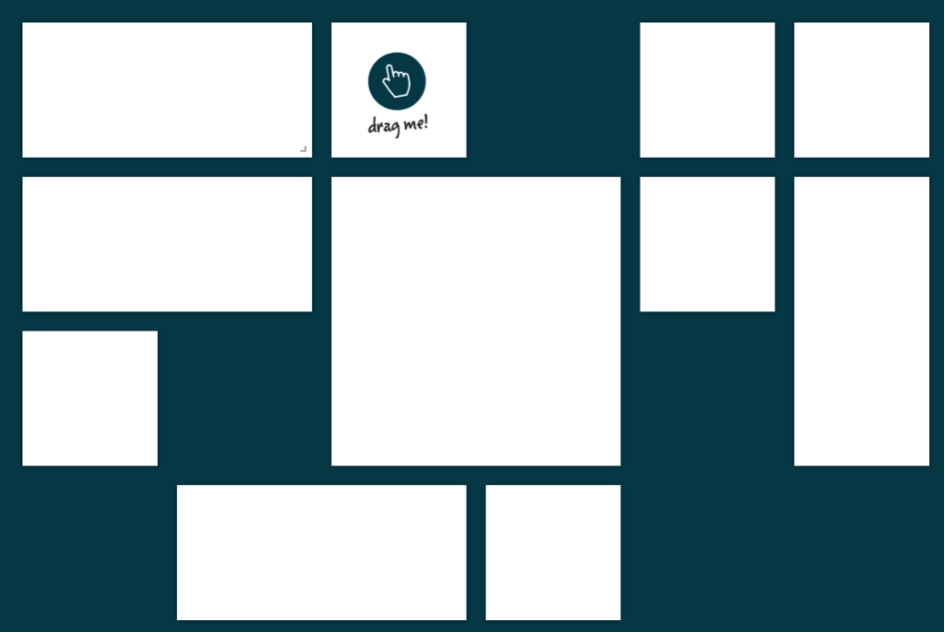
\includegraphics[width=0.5\textwidth]{pictures/matthieu/m_gridster.png}
	\caption{Démo d'une grille de widgets Gridster}
	\label{w1}
\end{figure}

Nous retrouvons sur cet aperçu de Gridster les principales fonctionnalités recherchées.

\subsection{Impression de la page de dashboard}

Afin de présenter des résultats clairs à leur entreprise, les utilisateurs de VMProject ont besoin d’avoir une version papier de ce tableau de bord, il faut donc qu’il puisse être imprimable. Cette demande a été rajoutée en fin de projet, nous allons voir par la suite comment nous avons réalisé cela.

\chapter{Réalisation et résultats}

	\section{Découverte du code}
Une fois la phase de conception terminée, nous avons pu découvrir le code qui fait fonctionner VMProject. Cette étape était assez conséquente car VMProject n’est pas si simple à comprendre. En effet, VMProject est une application qui a été développée par beaucoup de développeurs différents au cours des dernières années, et chaque développeur a codé avec sa propre logique. Cela a rajouté de la complexité à notre projet en plus de la documentation sur le code plutôt incomplète. Mais il faut tirer un avantage de cela, car cela a été très formateur pour nous.\\

 Pour comprendre le code il nous a fallu intégrer le principe de routes de MVC de l'application ou encore comprendre où et comment le code devait être modifié. Cependant, après une bonne semaine de découverte et de compréhension du code, nous étions prêts à démarrer le développement de notre dashboard. Ci-dessous le schéma présente l'architecture du code de VMProject et dans quels dossiers nous travaillons.\\

%schéma dossiers travail

VMProject est une application qui est développée en PHP pour la partie back-end. L'équipe de développement a développé un framework MVC hybride en interne pour supporter l'architecture de notre application web, sauf que comme le logiciel est très étendu, les versions de différentes parties du code ne sont pas forcément à jour. De notre côté nous avons donc aussi dû développer en PHP comme nous le verrons plus tard pour les différentes requêtes au back-end et à la base de données que nous avons faites.\\

Concernant la base de données, elle tourne sur un moteur MySQL qui est très intéressant. En effet, VMProject est conçu de telle manière que dès qu'une personne souhaite créer un projet et ajouter des utilisateurs dessus, elle créée dans la base de données MySQL une nouvelle base de données, appelée instance VMProject. Ainsi les données de chaque \emph{super-utilisateur} sont séparées.\\

Pour le front-end et donc la partie client cela est fait de manière logique en HTML et CSS via des templates qui sont interprétés par le moteur de rendu du framework MVC mais aussi avec du javascript. Il est très important de souligner que VMProject est une très grosse application javascript qui fait donc appel à beaucoup de requêtes asynchrones en Ajax. Deux librairies importantes sont utilisées sur l'application : ext.js et aussi jQuery 1.4 ; cette dernière version comme nous l'avons vu précédemment est un point important car à l'heure actuelle jQuery en est dans sa version 2.\\

La phase de découverte du code a longtemps été repoussée car il était inutile de se plonger dans le code sans développer quelque chose.\\
	\section{Développement}
	
	\subsection{Intégration du module de widget}
	
	Grister fonctionne sous forme de balises à inclure dans le HTML, elles sont ensuite traitées par le JavaScript et le CSS pour permettre son utilisation.
Pour être utilisé ce plugin, nécessite jQuery en version 1.7.1 au minimum et le fichier JavaScript de Gridster, or la version présente sur le serveur est plus ancienne.\\
	
	
La première idée à donc été de mettre à jour le site pour qu’il soit fonctionnel avec une version récente de jQuery, ce qui s'est révélé être un travail trop long au vu des erreurs rencontrées. Nous avons donc opté pour utiliser deux versions de jQuery en même temps.\\
	

VMProject utilise un moyen spécial pour inclure les bibliothèques JavaScript, au lieu de les importer directement sur la page HTML, elles sont importées depuis le PHP. En effet les fichiers à inclure sont écrits dans un tableau, et un script PHP ajoute les balises d’inclusions dans le HTML. Cependant, lorsque le site VMProject est appelé depuis Internet Explorer dans une version inférieure à la 8, un traitement spécial est effectué pour l’inclusion du JavaScript. Celui-ci est traité par un système qui concatène tous les fichiers les uns à la suite des autres, dans le but de réduire le nombre de caractères car Internet Explorer n’autorise qu’un nombre limité de caractères.\\
	
	\begin{figure}[H]
	\centering
	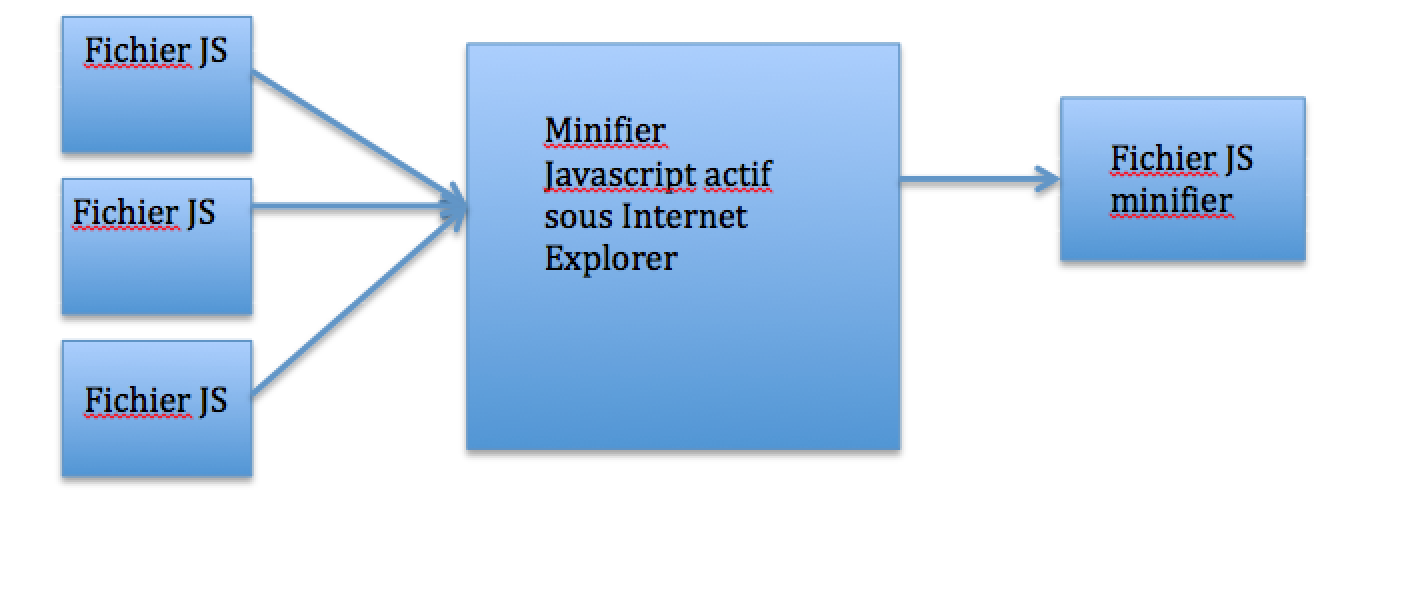
\includegraphics[width=1\textwidth]{pictures/matthieu/m_minifier.png}
	\caption{Schéma fonctionnement minifier}
	\label{w2}
\end{figure}
	
Différentes méthodes ont été testées pour ajouter jQuery 1.7.1 au projet, sans interférer avec les autres parties de VMproject.

L’élément clé pour faire fonctionner en parallèle deux versions de jQuery réside dans le fait de les nommer différemments lors de l’importation. Pour ceci on utilise la méthode noConflict() de jQuery, qui retourne la version courante de jQuery ET force \$ -- variable jQuery -- à ne plus pointer vers jQuery. Il faut donc inclure la version nécessaire 1.7.1, utiliser noConflict, et inclure Gridster.

Cependant, cette méthode fonctionne que pour Firefox et Chrome, en effet sur Internet Explorer, quand le minifier est appelé la double version de jQuery ne fonctionne pas. Il a donc finalement fallu faire les importations directement dans le HTML pour intégrer Gridster à VMproject.

	\subsection{Réalisation du calendrier}
	
Afin de se repérer temporellement dans le projet, il fallait trouver un moyen d’afficher les informations importantes dans un repère temporel.\\

Nous avons donc décidé de créer un calendrier de 4 semaines glissantes. Il fallait ensuite savoir quelles informations représenter et sous quelle forme. Après une étude sur les critères importants, sont ressorties 3 informations :\\
	
	\begin{itemize}
\item	Les jalons, représentent la date et le nom du jalon
\item	Les réunions, indiquent la date et le nom de la réunion
\item	Les livrables, indiquent la date de la validation du livrable, ou la date de fin projetée de la tâche si le livrable n’a pas été validé.\\
	\end{itemize}


\subsubsection{Comment récupérer les données ?}
La principale difficulté de ce widget est de récupérer les données concernant les différents évènements à venir.\\
	
\begin{figure}[H]
	\centering
	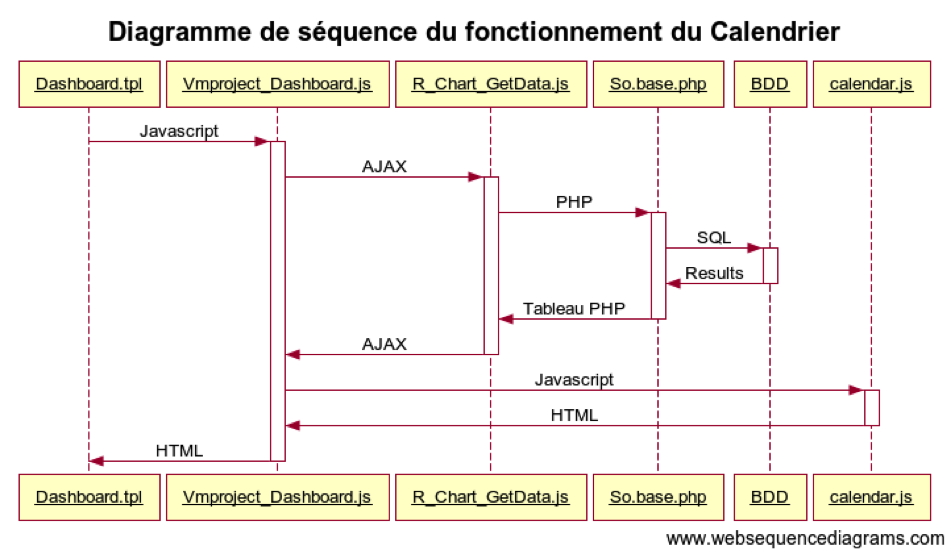
\includegraphics[width=1\textwidth]{pictures/matthieu/m_sequence.png}
	\caption{Graphe de séquence sur la récupération de données pour le calendrier}
	\label{m1}
\end{figure}
	
	Ce diagramme de séquence résume les échanges internes de cette partie. Ainsi lors de l’appel de la page "Tableau de bord", le fichier principal vm\_project\_dashboard est appelé. En découle ensuite plusieurs échanges avec la base de données et avec le fichier Javascript du calendrier.\\
	
Pour récupérer les réunions il suffit d’interroger la base de données, puis de manipuler l’information pour la transmettre d’un langage à un autre. Il en va de même pour les livrables et les jalons.\\
\subsubsection{Comment présenter les données ?}
L’idée principale était d’afficher 4 semaines, où chaque ligne représente une donnée.\\
\begin{figure}[H]
	\centering
	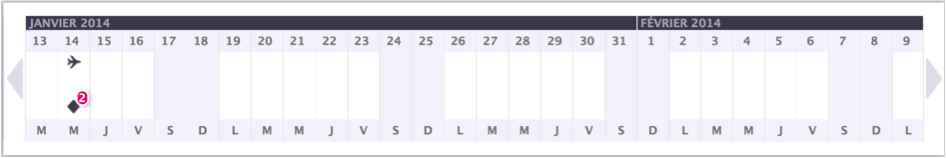
\includegraphics[width=1\textwidth]{pictures/matthieu/m_calendar_1.png}
	\caption{Calendrier, 4 semaines}
	\label{m2}
\end{figure}
	Après les deux premières lignes représentant le repère temporel on retrouve les livrables symbolisés par un petit avion. Les réunions ensuite, puis les jalons.\\

Il est possible que plusieurs éléments d’un même type ait lieu au même moment, dans ce cas une petite pastille apparaît indiquant le nombre d’éléments superposés. Lors du passage de la souris, un détail des événements apparaît dans une infobulle. On remarque ici que pour les réunions, le nom de la réunion et sa date apparaissent.\\
	
\begin{figure}[H]
	\centering
	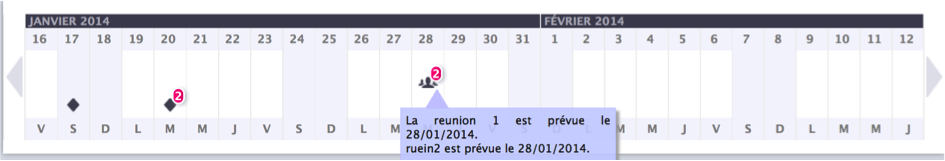
\includegraphics[width=1\textwidth]{pictures/matthieu/m_calendar_2.png}
	\caption{Calendrier, plusieurs évènements}
	\label{m3}
\end{figure}
	
	L’une des difficultés rencontrées dans la présentation des données, a été de gérer les cas limite. Comme par exemple quand on affiche que très peu de jours d’un mois, le nom du mois ne peut pas être affiché completement. Il faut alors calculer au préalable le nombre de jours prévus dans le mois à afficher et si celui-ci est trop petit, alors on n’affiche qu’une partie du mois.\\

Voici un aperçu montrant comment le problème a été résolu :\\
	
	\begin{figure}[H]
	\centering
	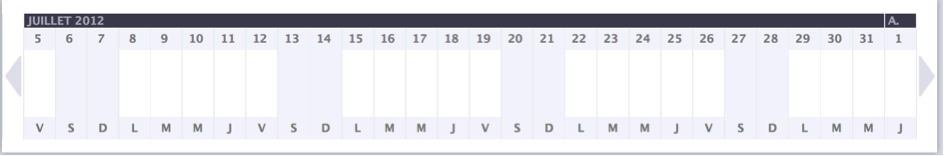
\includegraphics[width=1\textwidth]{pictures/matthieu/m_calendar_3.png}
	\caption{Calendrier, résolution des mois trop grands}
	\label{m4}
\end{figure}

	\subsection{Réalisation des graphes d'avancement/charges/budget}
	
	\subsubsection{Implantation dans la page}
	
	Comme expliqué dans le chapitre de conception, ces trois graphiques ont pour objectif respectif de représenter l’avancement, le budget et les charges pour un projet ou une tâche ou sous-tâche de celui-ci, et sur une période donnée. Bien que représentant des données de nature différente, ils sont assez similaires au niveau du développement étant donné que le type de représentation graphique utilisé est identique. Ils ont donc été conçus de la même manière en s’appuyant sur les mêmes fonctions. Tous trois dépendent de deux sélecteurs situés dans la barre située plus haut : un sélecteur de tâche et un sélecteur de période. La modification d’un sélecteur doit changer dynamiquement les données affichées par les trois graphes. Toutefois, les deux fonctionnent de manières différentes en termes de récupération des données :\\
	
\begin{itemize} 
\item A l’initialisation, chacun des graphes est créé avec comme paramètre l’ensemble des données nécessaires relatives à toutes les tâches du projet sur toute la durée de la tâche. Pour modifier le graphe, il suffit ensuite de faire appel à la fonction « change » du graphe qui actualise celui-ci en connaissant seulement l’identifiant de la tâche
\item	Concernant la période en revanche, un appel à la base de données et nécessaire à chaque modification du critère de recherche ; en effet, il apparait impossible de prévoir à l’avance tous les cas possibles, sachant que l’utilisateur peut sélectionner manuellement les dates de début et de fin de période. Néanmoins, cette requête en base de données n’est pas faite directement depuis la méthode du graphique, mais depuis la classe VMProject\_Dashboard qui centralise toutes les données relatives aux graphes.\\
\end{itemize}
Finalement, chaque graphe possède sa propre classe mais est averti par une classe commune lors d’un changement de critère d’affichage, avec en paramètre les données à afficher ou un indicateur sur celles-ci. Etant donné que les trois jauges sont relativement similaires, nous avons également choisi dans un souci de clarté du code de regrouper toutes les méthodes communes à la création des différents éléments graphiques (arcs, cercles, couleurs, vitesses…) dans une seule classe accessibles par les classes des trois graphes : la classe ManagerDataPie. Le fonctionnement général est décrit dans la figure \ref{c3}.  

	\subsubsection{Données représentées}

Un bref rappel du logiciel VMProject est nécessaire ici : celui-ci se base sur trois modes de vision du projet : le réel, le prévu et le projeté. Le réel correspond comme son nom l’indique à la réalité, c’est-à-dire à ce qui a été effectivement fait. Le prévu s’appuie sur les prévisions rentrées dans le logiciel par l’utilisateur au moment du planning prévisionnel ; il modélise là où le projet devrait en être. Le mode projeté calcule au vu de ce qui a été réalisé et ce qui a été prévu de faire une estimation de la durée ou de la quantité totale. Ces trois modes suivent un code couleur visible en haut à droite de la dashboard, qui est le suivant :\\

	\begin{figure}[H]
	\centering
	
\includegraphics[width=0.5\textwidth]{pictures/clement/c4.png}
	\caption{Légendes des couleurs de la page}
	\label{c4}
\end{figure}

En ce qui concerne le graphe de budget, l’idée est ici d’indiquer à l’utilisateur de manière très rapide si le budget alloué à la tâche concernée est dépassé ou s’il peut encore se permettre des dépenses. Avec l’utilisation d’une jauge, la lisibilité est facile et rapide. Afin de représenter les trois modes sur le même graphe, nous utilisons plusieurs jauges concentriques de rayons différents accompagnées de diverses indicateurs chiffrés. Tout en conservant le couleur, nous affichons et même superposons toutes les données pour une meilleure compréhension et pour rendre possible la comparaison. Détaillons le cas de l’exemple présenté ci-dessous (fig. \ref{c5}).\\

\begin{figure}[H]
	\centering
	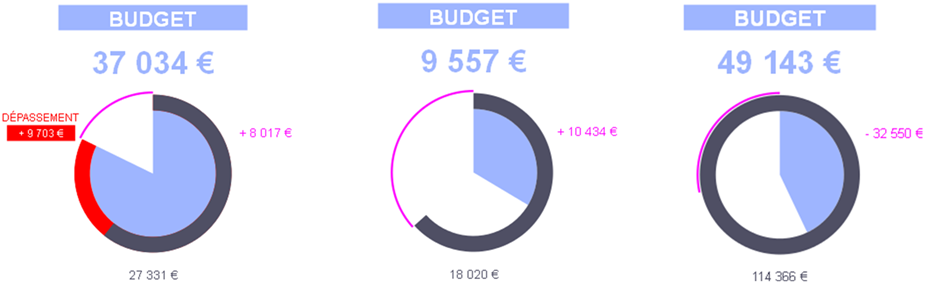
\includegraphics[width=1\textwidth]{pictures/clement/c5.png}
	\caption{Exemples des graphes indicateurs}
	\label{c5}
\end{figure}

Plusieurs faits sont notables ici.\\
Pour le graphe de gauche :\\
\begin{itemize}
\item	Le budget dépensé s’élève actuellement à 37 034 \euro{}.
\item Le budget prévu pour cette tâche était initialement de 27 331  \euro mais est clairement dépassé, ce qui saute d’ailleurs directement aux yeux grâce à la couleur rouge. On note que le dépassement de budget est pour le moment de 9 703  \euro{}.
\item On peut encore s’attendre à 8 017  \euro{} de dépenses sur cette tâche.
Pour le graphe central :
\item Le budget prévu de 18 020  \euro{} n’est pas encore dépassé mais les prévisions estiment qu’il le sera dans le futur pour un surcoût de 10 434  \euro{}.
Pour le graphe de droite : 
\item La valeur du projeté est précédée d’un signe « - » ce qui signifie que le projeté est inférieur au prévu : des économies devraient être effectuées, à hauteur de : 114 366  \euro{} - 32 550  \euro{} (soit 81816  \euro{}). La jauge du projeté peut donc être en addition du prévu, ou en soustraction de celui-ci.
Graphiquement, les proportions relatives des données, bien que non indiquées numériquement, sont très visibles. Ces graphes regroupent une grande quantité de données et sont pourtant très lisibles. Le graphe de charges fonctionne exactement de la même manière que celui de budget, au détail près qu’il affiche l’avancement du projet en termes de charges en jours/hommes. Il ne tient pas compte du temps, seulement de la charge de travail effectuée/qui aurait dû être effectuée/restant à effectuer selon le calcul du logiciel. Nous ne détaillerons pas le fonctionnement détaillé étant donné qu’il est vraiment similaire au graphe de budget pour la lecture et la compréhension.\\
\end{itemize}
Concernant le graphe d’avancement, l’objectif est de donner une idée à l’utilisateur de son avancée dans le projet ou dans la tâche en termes de temps.  Un projet est avant tout un délai à respecter et donc une course contre le temps. Il se distingue du graphe de charge car ce dernier tient compte du travail effectué en jours/hommes, alors qu’ici la quantité de travail n’intervient pas dans la jauge : la valeur représentée est le temps écoulé entre la première feuille de temps ajoutée sur la tâche et la dernière. Il est donc possible que pendant une longue durée, aucun travail ne soit accompli et pourtant le temps avance. Graphiquement, on retrouve les mêmes éléments que pour les deux graphes précédents, comme on peut le voir sur la partie gauche de la figure suivante :\\

\begin{figure}[H]
	\centering
	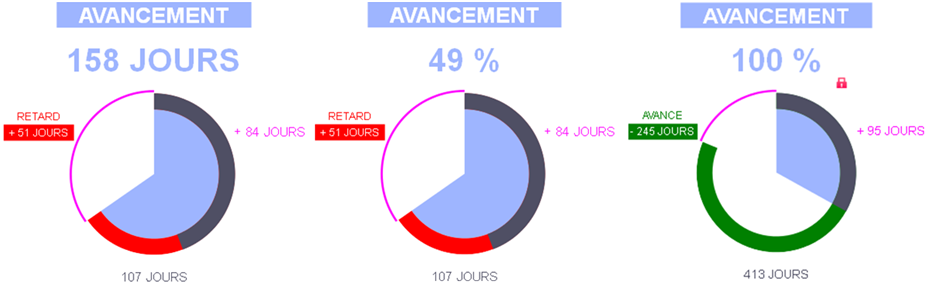
\includegraphics[width=1\textwidth]{pictures/clement/c6.png}
	\caption{Détails des exemples indicateurs}
	\label{c6}
\end{figure}

Toutefois, l’affichage de gauche n’est pas le principal : l’indication du temps réel passé (ici 158 jours) n’est visible qu’au passage de la souris sur la partie bleue du graphe. En temps normal, c’est le pourcentage d’avancement du projet qui est écrit à l’écran (comme sur le graphe du milieu). On peut immédiatement remarquer que ce pourcentage ne correspond pas au remplissage de la jauge ; ceci s’explique par le fait que l’indicateur en pourcentage soit la valeur d’avancement global de la tâche sélectionnée, et non pas d’avancement temporel. Ce choix a été fait pour permettre à l’utilisateur de se rendre compte du temps qu’il lui reste avant la fin prévue de la tâche et de la quantité de travail qu’il reste à faire. Dans notre cas, la date de fin de tâche est déjà dépassée et pourtant seulement la moitié du travail a été effectuée ; la tâche a déjà 51 jours de retard, et le logiciel a prévu qu’il y aurait encore besoin de 84 jours pour la terminer…  En cas d’avance temporelle à la fin d’un projet ou d’une tâche, la partie rouge du retard prend une couleur verte pour l’avance, comme on peut le voir sur la partie droite de la figure ci-dessus.\\
VMProject permet de forcer une valeur, c’est-à-dire de la rentrer manuellement même si elle est contraire aux calculs ou aux prévisions du logiciel. Par exemple, si moins d’heures que prévues ont été consacrées à la terminaison d’une tâche, celle-ci ne sera pas considérée comme finie par le logiciel alors qu’elle l’est en réalité. L’utilisateur peut alors placer l’avancement de la tâche à 100\% et le déclarer comme terminer. Ces cas de forçage provoquent des incohérences graphiques, et nous affichons donc un petit cadenas rose pour le signaler avec une légende en bas du widget au passage de la souris sur le cadenas, comme on peut le voir sur la figure suivante :\\

\begin{figure}[H]
	\centering
	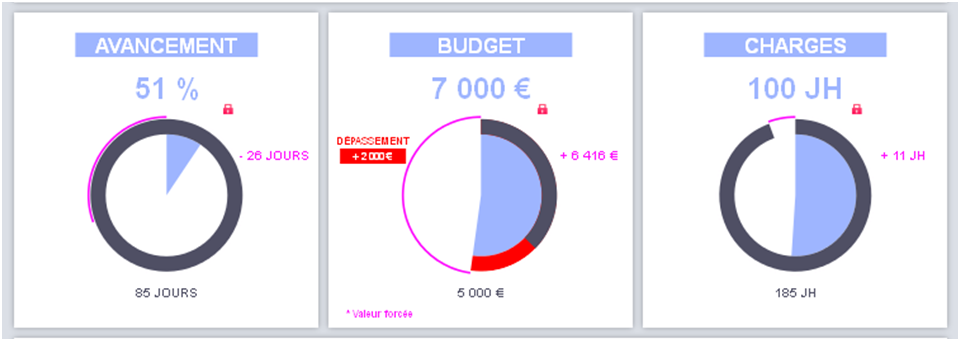
\includegraphics[width=1\textwidth]{pictures/clement/c7.png}
	\caption{Données forcées affichage d'un cadenas}
	\label{c7}
\end{figure}

	\subsubsection{Outils graphiques et techniques}
	
	Comme précisé dans les choix techniques, nous utilisons la librairie D3.js pour construire nos graphes. Le concept de jauge était déjà défini dans la bibliothèque : le principe est en fait de définir dans un premier temps un cercle de largeur non nulle (écart entre deux cercles de rayons différents) que nous appellerons arc, et dans un second temps de choisir un angle à colorier. Pour superposer les différents modes (réel, prévu, projeté), il a donc fallu superposer les jauges selon un ordre d’affichage précis ; en effet, le retard est représenté sur le même arc que le prévu. La valeur des données à afficher est également à prendre en compte. A titre d’exemple, voici la chronologie d’affichage des différentes jauges pour un graphe d’avancement quelconque :\\
	
	\begin{figure}[H]
	\centering
	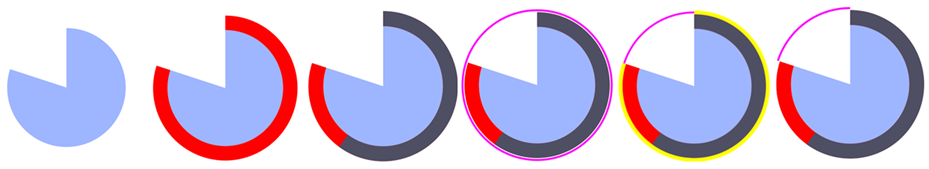
\includegraphics[width=1\textwidth]{pictures/clement/c8.png}
	\caption{Différents arcs de cercles choisis}
	\label{c8}
\end{figure}

A la 5\up{ème} étape, la couleur jaune a été ajouté artificiellement afin de rendre compte de la dernière jauge mise en place afin de limiter la jauge de projeté.

	\subsubsection{Difficultés rencontrées}
	
	La phase de développement concernant ces trois graphes s’est déroulée en trois étapes : dans un premier temps, l’aspect graphique a été mis en avant avec un développement en statique (les données utilisées pour alimenter les graphes étaient codées en dur), puis la connexion avec les données de la base de VMProject a été établie, et enfin l’affichage a été modifié afin de traité tous les cas possibles. \\
	
La difficulté de la première étape a été de se familiariser avec D3.js et le format SVG ; cette librairie utilise ce format pour l’affichage des graphes. Le paramétrage et l’utilisation des critères graphiques ainsi que l’ajout de fonctionnalités dynamiques (visibles à chaque changement de tâche notamment, avec par exemple les transitions lors de l’évolution des graphes ou encore l’effet de rebond) ont demandé de nombreuses recherches et un certain nombre d’essais avant d’être fonctionnels. \\
	
La seconde étape a sans doute été la plus longue étant donné qu’il a fallu d’abord trouver dans la base les données à afficher, les calculer et leur donner le bon format, puis les connecter avec les graphes. En particulier, avec le sélecteur de période, on peut choisir une durée précise sur une tâche. Dans ce cas, pour le graphe de charges, il est obligatoire d’additionner toutes les feuilles de temps en base de données sur la période sélectionnée.\\
	
La troisième étape, bien que peu productive en quantité de code, a nécessité beaucoup de temps afin d’identifier les cas particuliers, de comprendre les erreurs et de les corriger. Dans les cas non représentables (toutes les valeurs à zéro par exemple), un message d’erreur est affiché, comme dans les graphes de budget de la figure \ref{c9}. Certaines configurations, présentées également dans la figure, paraissent vide de sens. C’est souvent le cas pour des tâches qui ne durent qu’une journée ou qui ont été créées mais inutiles et finalement considérées comme terminées.\\
	
		\begin{figure}[H]
	\centering
	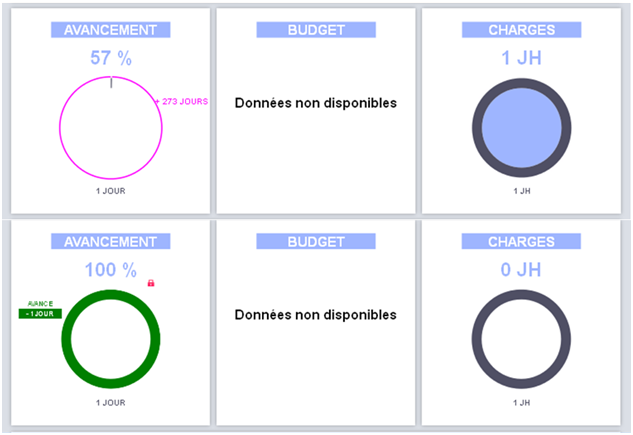
\includegraphics[width=1\textwidth]{pictures/clement/c9.png}
	\caption{}
	\label{c9}
\end{figure}

	\subsection{Réalisation du graphique de répartition}

\begin{figure}[H]
	\centering
	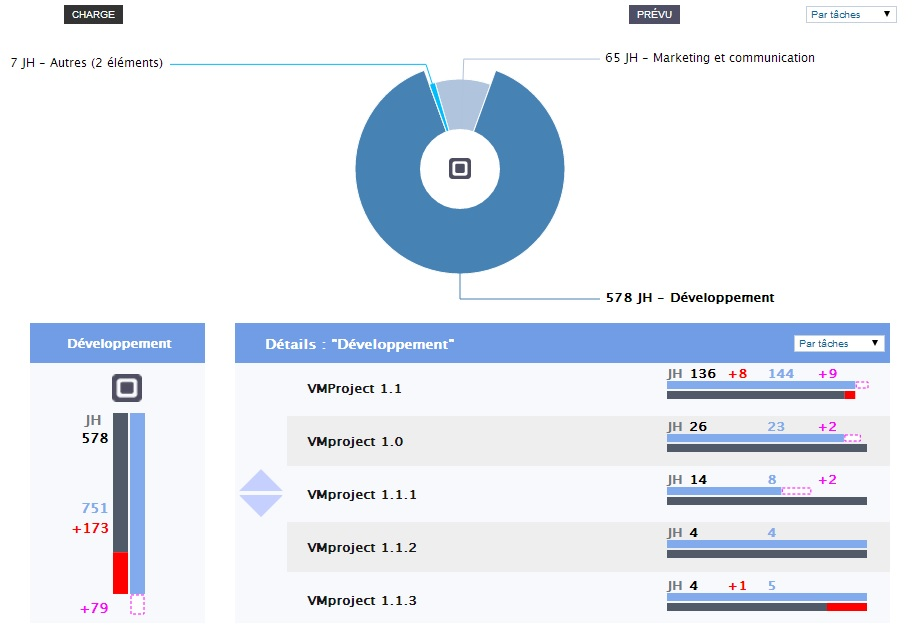
\includegraphics[width=1\textwidth]{pictures/realisations/repartition.jpg}
	\caption{}
	\label{17}
\end{figure}

Le graphique de répartition a été développé en local par Thibaut Zonca et Christophe Blefari a travaillé sur son intégration au tableau de bord en ligne (et donc à la connexion des données). Ce graphique étant assez complexe (nous n'avons pas tout compris pendant un certain temps), il a fallu découper son développement en plusieurs parties plus simples. \\

Notre code pour ce graphique est contenu dans une classe javascript. Les différentes parties du graphique sont tracées grâce à des appels de fonctions. Pour rendre possible la configuration rapide de paramètres importants, nous avons implémenté une configuration sous forme de dictionnaire dans cette classe.\\

Décomposition du graphique en éléments simples :\\

\begin{enumerate}
\item \textbf{Camembert}\\

\begin{figure}[H]
	\centering
	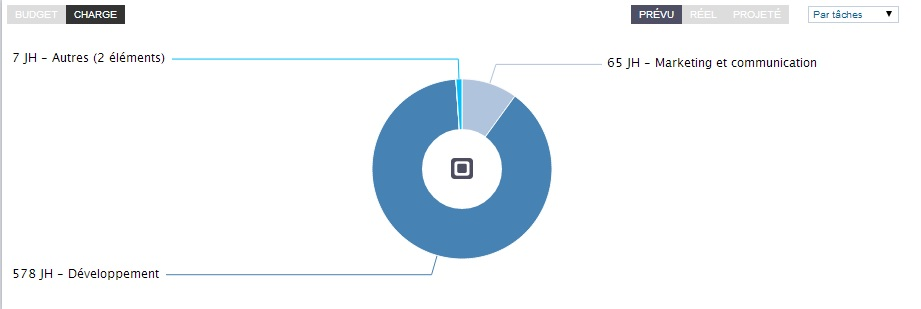
\includegraphics[width=1\textwidth]{pictures/realisations/camembert.jpg}
	\caption{Graphique de répartition}
	\label{18}
\end{figure}

La première étape a été de programmer le graphique principal, le camembert. Pour cela, la librairie D3.js a été utilisée comme pour nos autres graphiques; cette permet de faire des graphiques en SVG et bien plus encore. Grâce à D3.js, nous avons pu développer notre propre graphique qui propose aussi des effets agréables comme des transitions : en changeant de mode (prévu, réel, projeté), les parts de notre camembert sont recalculées et elles "glissent" automatiquement de manière fluide pour présenter les nouvelles données à afficher.\\

Cependant, certaines fonctionnalités ont demandé plus de réflexion : il est plus facile de se documenter sur la façon de construire un graphique de type camembert avec D3.js, que sur des points beaucoup plus précis qui sont ceux de notre projet industriel. C'est là que nous devons faire preuve d'imagination dans notre approche pour résoudre un problème par ses propres moyens. \\

Parmi ces points plus difficiles, il y a par exemple le traçage des traits pour qu'ils correspondent à ce que l'on peut voir sur la maquette de Versusmind (et aussi trivial que celà puisse paraître, la gestion des légendes n'est pas gérée de manière simple par D3.js). Le problème sera résolu après de longues séances d'essais, en calculant les coordonnées des lignes à tracer grâce à l'angle médian de chaque part. 
Autre point, les transitions entre les différents modes ont parfois posé problème, car la structure des données change (le nombre de tâches prévue peut être différent du nombre de tâche qui ont réellement été commencées) parfois entre les modes, ce que nous n'avions pas forcément prévu au départ.
Pendant un long moment, nous avions un autre problème d'affichage important lié aux légendes : lorsque des parts étaient très petites, les légendes de cette part et de ses parts voisines étaient souvent affichées à quelques millimètres d'écart seulement, ce qui rendait la lecture impossible. Problème contourné en créant une catégorie "Autres" regroupant les parts inférieures à un pourcentage donné; nous avons choisi 7\% pour un confort de lecture optimal.\\


\item \textbf{Détail (simple) de tâche / ressource}\\

\begin{figure}[H]
	\centering
	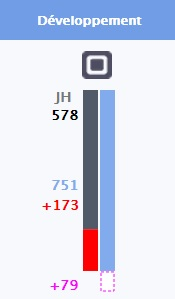
\includegraphics[width=0.3\textwidth]{pictures/realisations/detailTache.jpg}
	\caption{Detail de tâche}
	\label{19}
\end{figure}

Ensuite, la deuxième étape a été de développer le petit encart qui s'affiche au clic sur une part, donnant des informations sur la tâche ou ressource sélectionnée (toujours en terme de prévu, réel et de projeté). Encore une fois, le développement s'est fait grâce à D3.js pour tracer automatiquement ce petit graphique. Ce graphique a été plus rapide a développer que le camembert car il est moins complexe.\\

Par contre, il aura fallu plusieurs semaines trouver tous les petits bugs qu'il présentait, car le nombre de combinaisons de données et donc de possibilités d'affichages différents possibles générait de temps à autre une erreur qui n'avait pas encore été détectée.\\


\item \textbf{Détails (avancés) de tâche / ressource}\\

\begin{figure}[H]
	\centering
	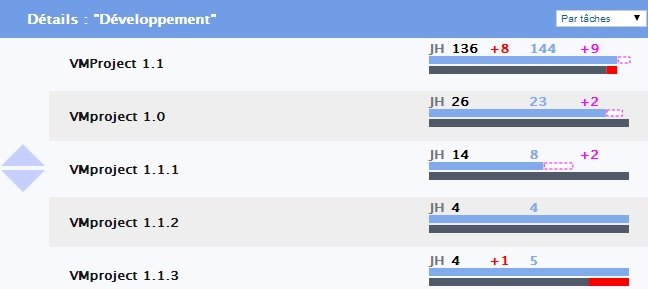
\includegraphics[width=1\textwidth]{pictures/realisations/detailsTache.jpg}
	\caption{Détails (avancés) d'une page}
	\label{20}
\end{figure}

La troisième étape a été de développer le grand encart, situé à droite du graphique de détail simple de tâche. Comme vous l'aurez remarqué, ce nouveau graphique est en fait composé de plusieurs petits graphiques simples de détails, mais orientés horizontalement.\\

Ce graphique affiche au choix, grâce au sélecteur situé en haut à droite du graphique :\\

\begin{itemize}
\item le détail des tâches composant la tâche sélectionnée
\item le détail des ressources composant la tâche sélectionnée
\item le détail des tâches qu'a effectué la ressource sélectionnée.\\
\end{itemize}


Intégration des graphiques sur le tableau de bord, connexion des données

Christophe, à toi de jouer !



Finalement, ce graphique complexe aura au total nécessité ?????????????? heures de travail, répartis sur 40 jours entre deux personnes.\\


%------------------------------------------------------------------------------------------------------------


\item \textbf{Réalisation du filtre de période}

\begin{figure}[H]
	\centering
	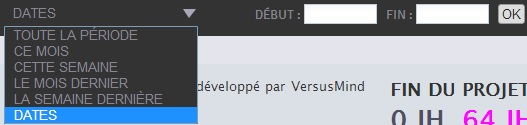
\includegraphics[width=1\textwidth]{pictures/realisations/filtrePeriode.jpg}
	\caption{Filtre de période}
	\label{21}
\end{figure}

Pour le réaliser, nous nous sommes mis d'accord avec nos encadrants industriels pour savoir quelles options proposer. Cinq options sont donc disponibles pour l'utilisateur de VMProject : le mois courant, la semaine courante, le mois dernier, la semaine dernière ou encore une période de son choix. Pour cette dernière option, il faut afficher un sélecteur de date sur la droite du filtre, comme illustré sur l'image ci-dessous.\\

\begin{figure}[H]
	\centering
	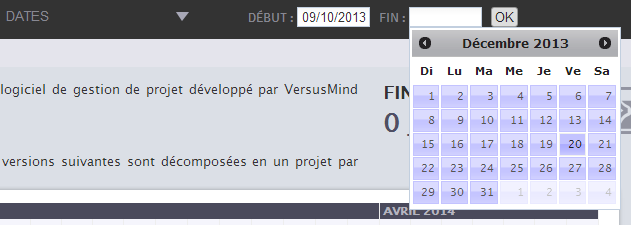
\includegraphics[width=1\textwidth]{pictures/realisations/filtrePeriodeDatepicker.png}
	\caption{Sélecteur de dates}
	\label{22}
\end{figure}

Ce filtre de période a donc été intégré au tableau de bord par Thibaut Zonca. L'intérêt de ce filtre est d'appliquer à tous les graphiques (qui ont été réalisés par différentes personnes) du tableau de bord la période sélectionnée. Pratique pour un chef de projet qui veut regarder ce qu'il s'est passé à un mois donné de l'année, ou bien lors de ses deux dernières semaines de vacances dans son projet, car ces périodes ne seraient pas été rapidement visualisables autrement.\\

Pour détailler le fonctionnement du filtre de période d'un côté plus technique, un calcul est fait en javascript pour déterminer le timestamp de l'option choisie. Le timestamp est un nombre qui désigne le nombre de secondes qui se sont écoulées depuis le 1er janvier 1970 à minuit; cela a par exemple pour avantage de faciliter la comparaison entre deux dates, car cela revient à faire la différence entre deux nombres entiers. Dans le cas de l'option de période personnalisable par l'utilisateur, le calcul est simple car les dates de début et de fin de période sont simplement données lorsque l'on clique sur le jour du calendrier (cf. fig \ref{22}); il faut donc simplement convertir ces deux dates du format "normal" au format timestamp. Dans le cas des quatre autres options, nous utilisons la date actuelle pour déterminer le mois et la semaine courant(e). Il reste donc à trouver le premier/dernier jour du mois ou de la semaine, et le tour est joué après conversion en timestamp.\\

Enfin, pour intégrer ce filtre aux autres graphiques, cela se traduit par une requête SQL sur la base de données de l'application dans le but d'extraire uniquement les informations (les ajouts ont aussi un timestamp) qui ont été ajoutées entre les deux dates que nous lui donnons en argument. Le calendrier a aussi nécessité des modifications car il doit toujours afficher une période d'un mois, il ne faut donc pas réduire sa taille lorsque l'on renseigne une période de deux semaines par exemple.\\


La réalisation de ce filtre a nécessité ?????????????? heures de travail.

\subsection{Page d'impression}

Pour rendre un site web imprimable il existe différentes solutions :\\

\begin{itemize}
\item	Créer une nouvelle feuille de style qui sera seulement appelée lors d’une demande d’impression.
\item Créer une nouvelle page dans un format imprimable (PDF / Image) ou seul les éléments important seront placés.
\end{itemize}

La solution d’exporter la page dans un autre format pour la rendre imprimable est beaucoup plus compliquée à mettre en œuvre et demande une charge de travail élevée, en revanche elle permet une mise en page précise qu’on ne pourrait pas avoir avec une autre méthode. Nous avons donc opté pour la première solution, à savoir créer une nouvelle feuille de style qui sera appelé que lors de l’impression. Cette fonctionnalité était déjà implantée sur les autres pages du site, nous devions donc faire attention de ne pas changer la version imprimable des autres pages.\\

\subsubsection{Comment choisir quel élément afficher ?}
Très vite nous nous sommes heurté à un problème. En effet nous essayons d’afficher les blocs, qu’on souhaitait faire apparaître dans la version imprimable, en spécifiant leur propriété display à block. Cependant rien ne s’affichait.\\

Nous avons donc recherché pourquoi rien ne s’affichait. Avant d’appeler la feuille de style ne notre page, le CSS principal était appelé en premier et forçait l’affichage de toute les div dans le html à none.\\

La propriété none de CSS est récursive, ce qui veut dire que si un élément à un fils à une propriété différente elle ne sera pas appliqué car none prendra le dessus.Ainsi pour afficher un élément enfant, nous devons afficher tous les éléments parents. Voici un aperçu de la façon d’on nous avons implémenter cette idée :\\

\begin{figure}[H]
	\centering
	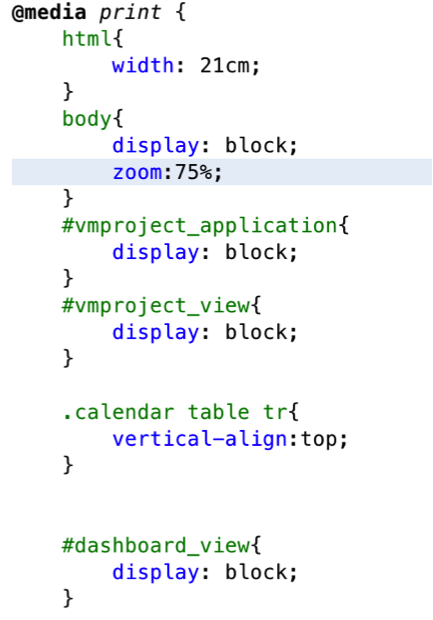
\includegraphics[width=0.3\textwidth]{pictures/matthieu/m_css_imprimabe.png}
	\caption{Extrait du code CSS}
	\label{m6}
\end{figure}

L’inscription « @media print » qui permet préciser le type de média nous indique que nous voulons choisir la vue impression. On remarque ensuite que pour afficher la balise vmproject\_view, nous sommes obligé d’appliquer la propriété block à cet élément ainsi qu’aux éléments parents : vmproject\_application et body.\\

Il en résulte une page épurée, sans le menu de latérale gauche, ni le menu supérieur (cf. fig \ref{m7}).

\end{enumerate}
	
	\section{Synthèse}
	
	\section{Résultat}
	

\chapter*{Conclusion}

En conclusion, concernant les chiffres à ce jour, nous avons passé environ 200 heures sur le projet dans sa globalité, que ce soit pour les tâches de conception mais aussi pour la gestion de projet. Comme nous l’avons expliqué précédemment la phase de conception s’est avérée plus ardue que prévue, c’est pourquoi notre projet a pris du retard et que nous en sommes à seulement 20\% de l’avancée globale. Mais maintenant que le développement est lancé nous allons avancer plus rapidement et tenter de rattraper ce retard.\\

Fiers de ces 200 heures de travail réalisés nous pouvons toutefois tirer des conclusions sur le projet, nous avons déjà étendu nos connaissances dans plusieurs domaines. Comme nous n’avions jamais commencé de projet de cette envergure, nous avons ainsi découvert le lancement d’un projet, mais aussi la phase très importante d’état de l’art, et celle de conception. Humainement nous avons aussi découvert le travail en équipe, puisque qu’en règle générale nous nous réunissions pour travailler et réfléchir ensemble. Cette expérience de travail en équipe sera un point important à mettre en avant de nos expériences passées dans notre vie professionnelle. \\

Nous avons aussi déjà acquis de l’expérience en développement, en effet il est à noter que l’application VMProject est une application à forte complexité ; beaucoup de développeurs d’horizons différents ont collaboré dessus et la profondeur du code est grande. Ainsi l’expérience de se plonger dans le code d’autrui a été une tâche difficile mais très formatrice. Cela nous a rendu tout de suite plus critique sur le travail à réaliser et sur l’obligation de rendre notre code compréhensible, simple et évolutif.\\

Il est évident qu’un projet de cette taille ne peut pas se dérouler sans embuches surtout dans le cas où c’est le premier de cette taille mais aussi qu’il n’est pas le seul projet que nous devons réaliser dans l’année. Ainsi nous nous sommes demandés, dans l’optique de nous améliorer, comment nous referions certaines tâches si nous recommencions le projet. \\

Comme il a été précisé précédemment la phase de conception a été difficile car nous ne savions pas ce que souhaitait l’entreprise dans sa dashboard, donc nous avons perdu beaucoup de temps. Cela a été sûrement dû au fait que l’étape de benchmark des concurrents s’est avérée complexe et que nous n’avons pas réussi à en tirer des conclusions intéressantes.\\

Une chose est sûre, nous avons déjà énormément appris sur la conduite d’un projet, que ce soit sur le plan humain ou sur le plan technique. Il est évident que ce projet industriel sera pour nous une très bonne expérience à mettre en avant dans le futur notamment dû à l’utilisation de technologies web comme HTML5 et le SVG qui sont fondatrices du web de demain.\\
\addcontentsline{toc}{chapter}{Conclusion}

\renewcommand{\appendixtocname}{Annexes} 
\begin{appendices}
\titlespacing*{\chapter}{0pt}{-0.8in}{20pt}

	\chapter{SquizAnalytics}

	\begin{figure}[!h]
	\centering
	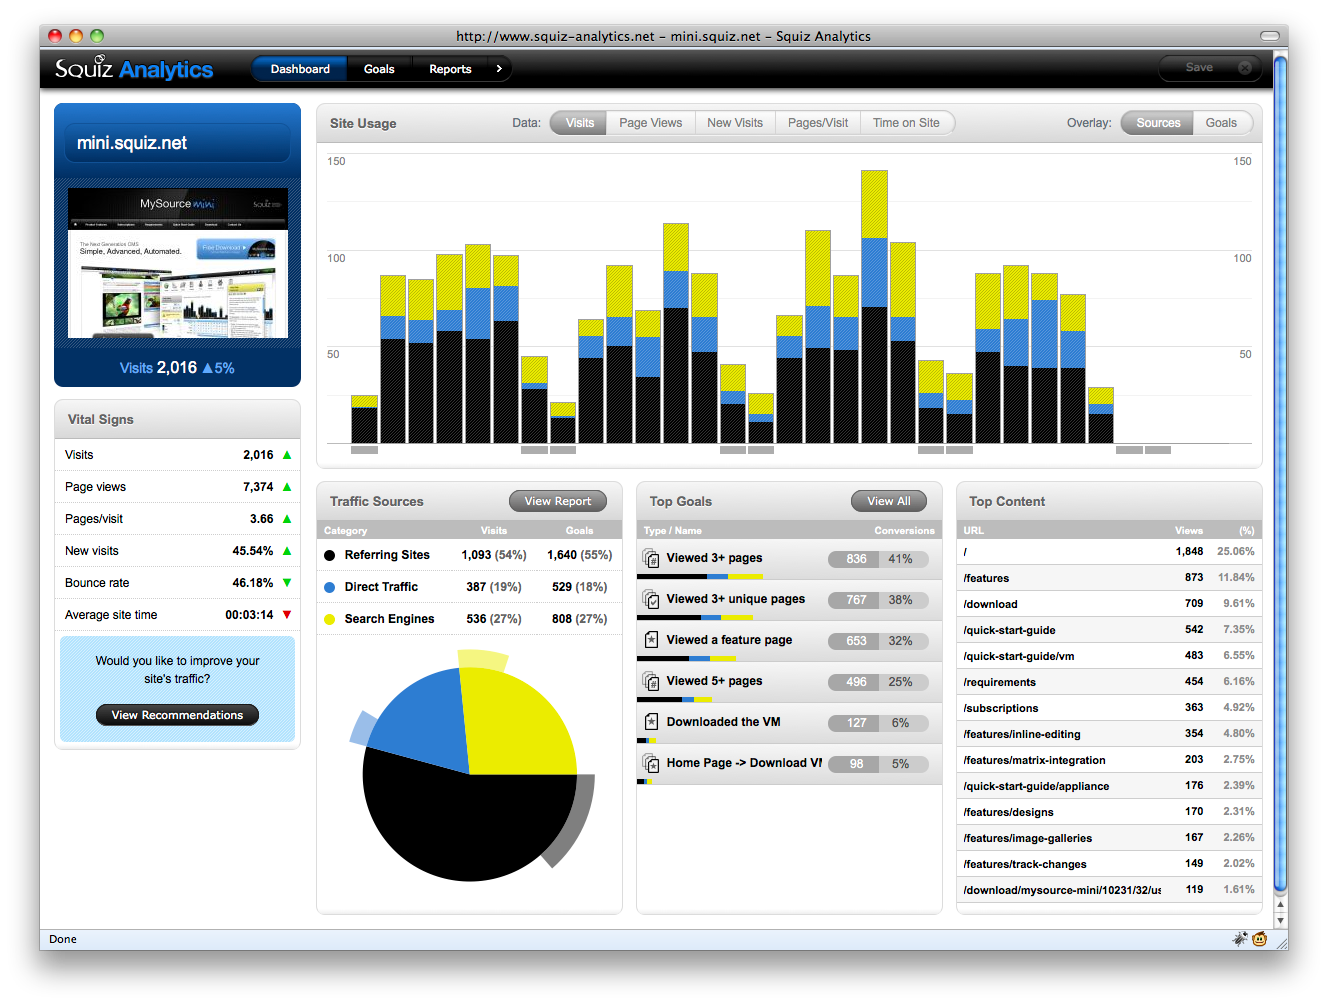
\includegraphics[width=1\textwidth]{pictures/squiz.png}
	\caption{Logiciel de GP Squiz Analytics}
	\label{a1}
\end{figure}
	
	\chapter{iGoogle}
	
	\begin{figure}[!h]
	\centering
	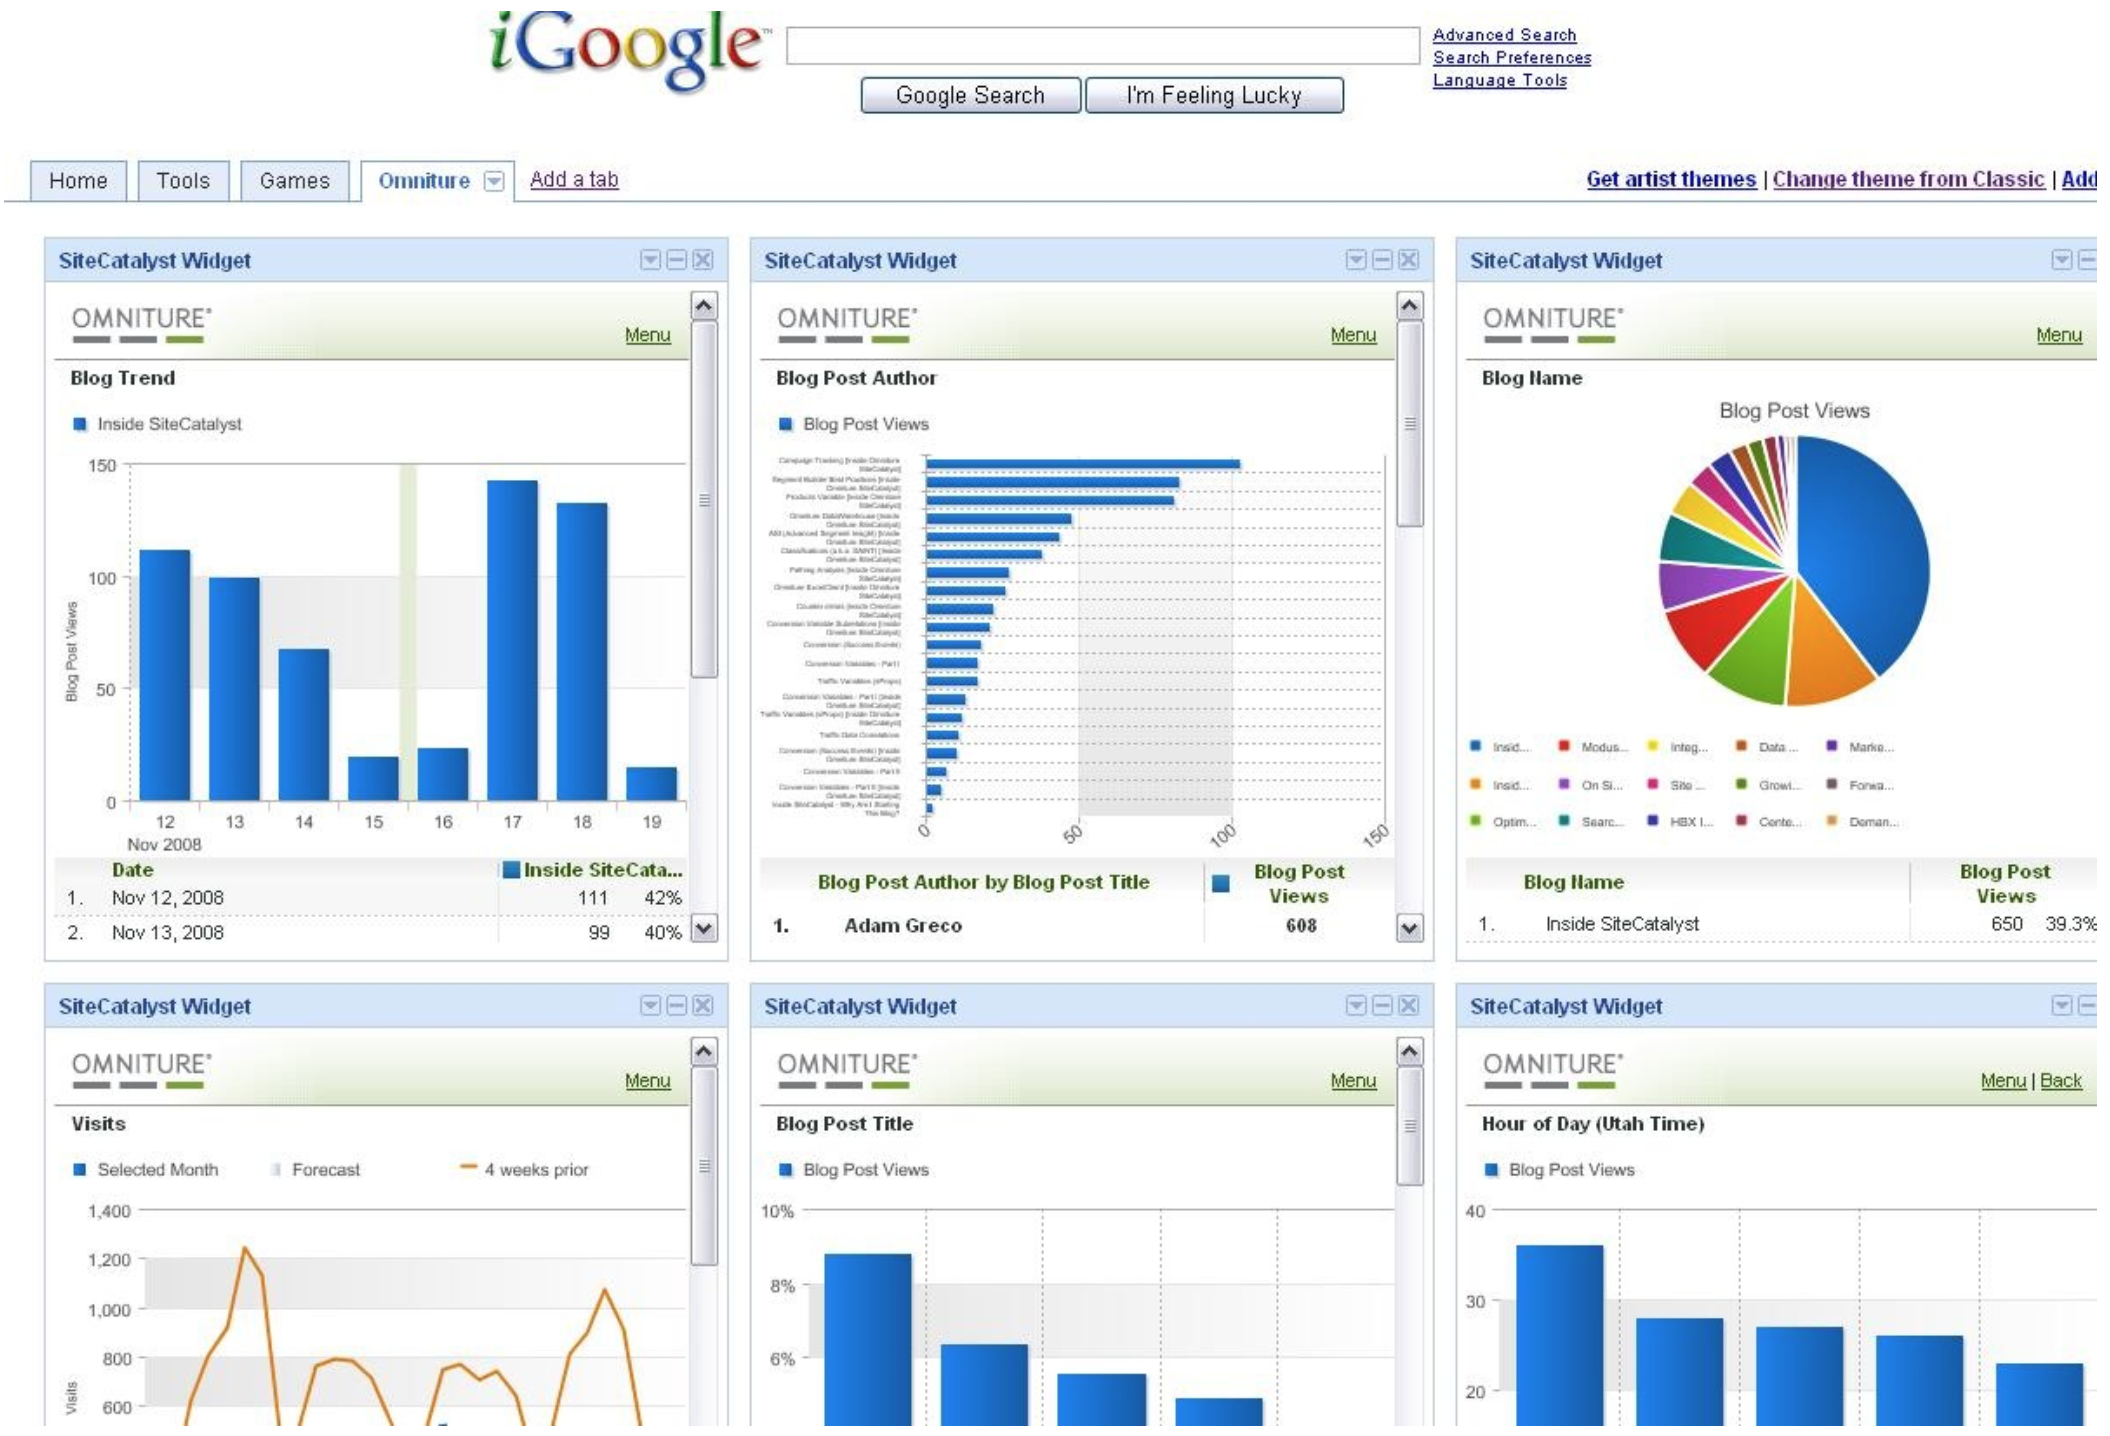
\includegraphics[width=1\textwidth]{pictures/igoogle.png}
	\caption{Ancienne page de iGoogle}
	\label{a2}
\end{figure}
	
	\chapter{Maquette complète proposée}
	
	\begin{figure}[H]
	\centering
	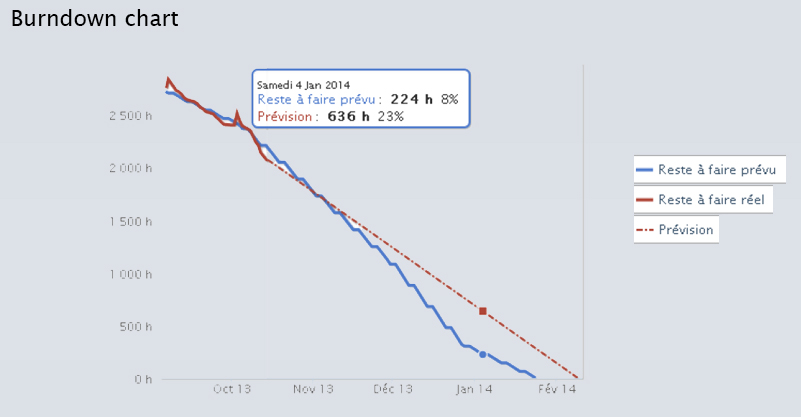
\includegraphics[width=1\textwidth]{pictures/notreMaquette/burndown.jpg}
	\caption{Burndown chart}
	\label{10}
\end{figure}

\begin{figure}[H]
	\centering
	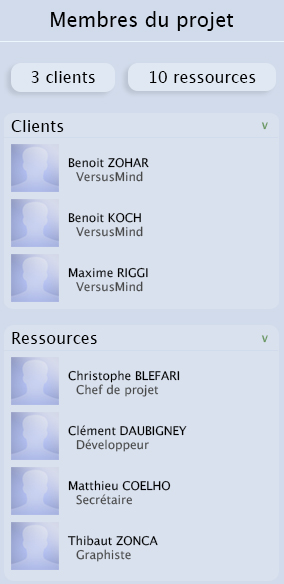
\includegraphics[width=0.3\textwidth]{pictures/notreMaquette/barreMembres.jpg}
	\caption{Barre des membres}
	\label{11}
\end{figure}
	
	\begin{figure}[!h]
	\centering
	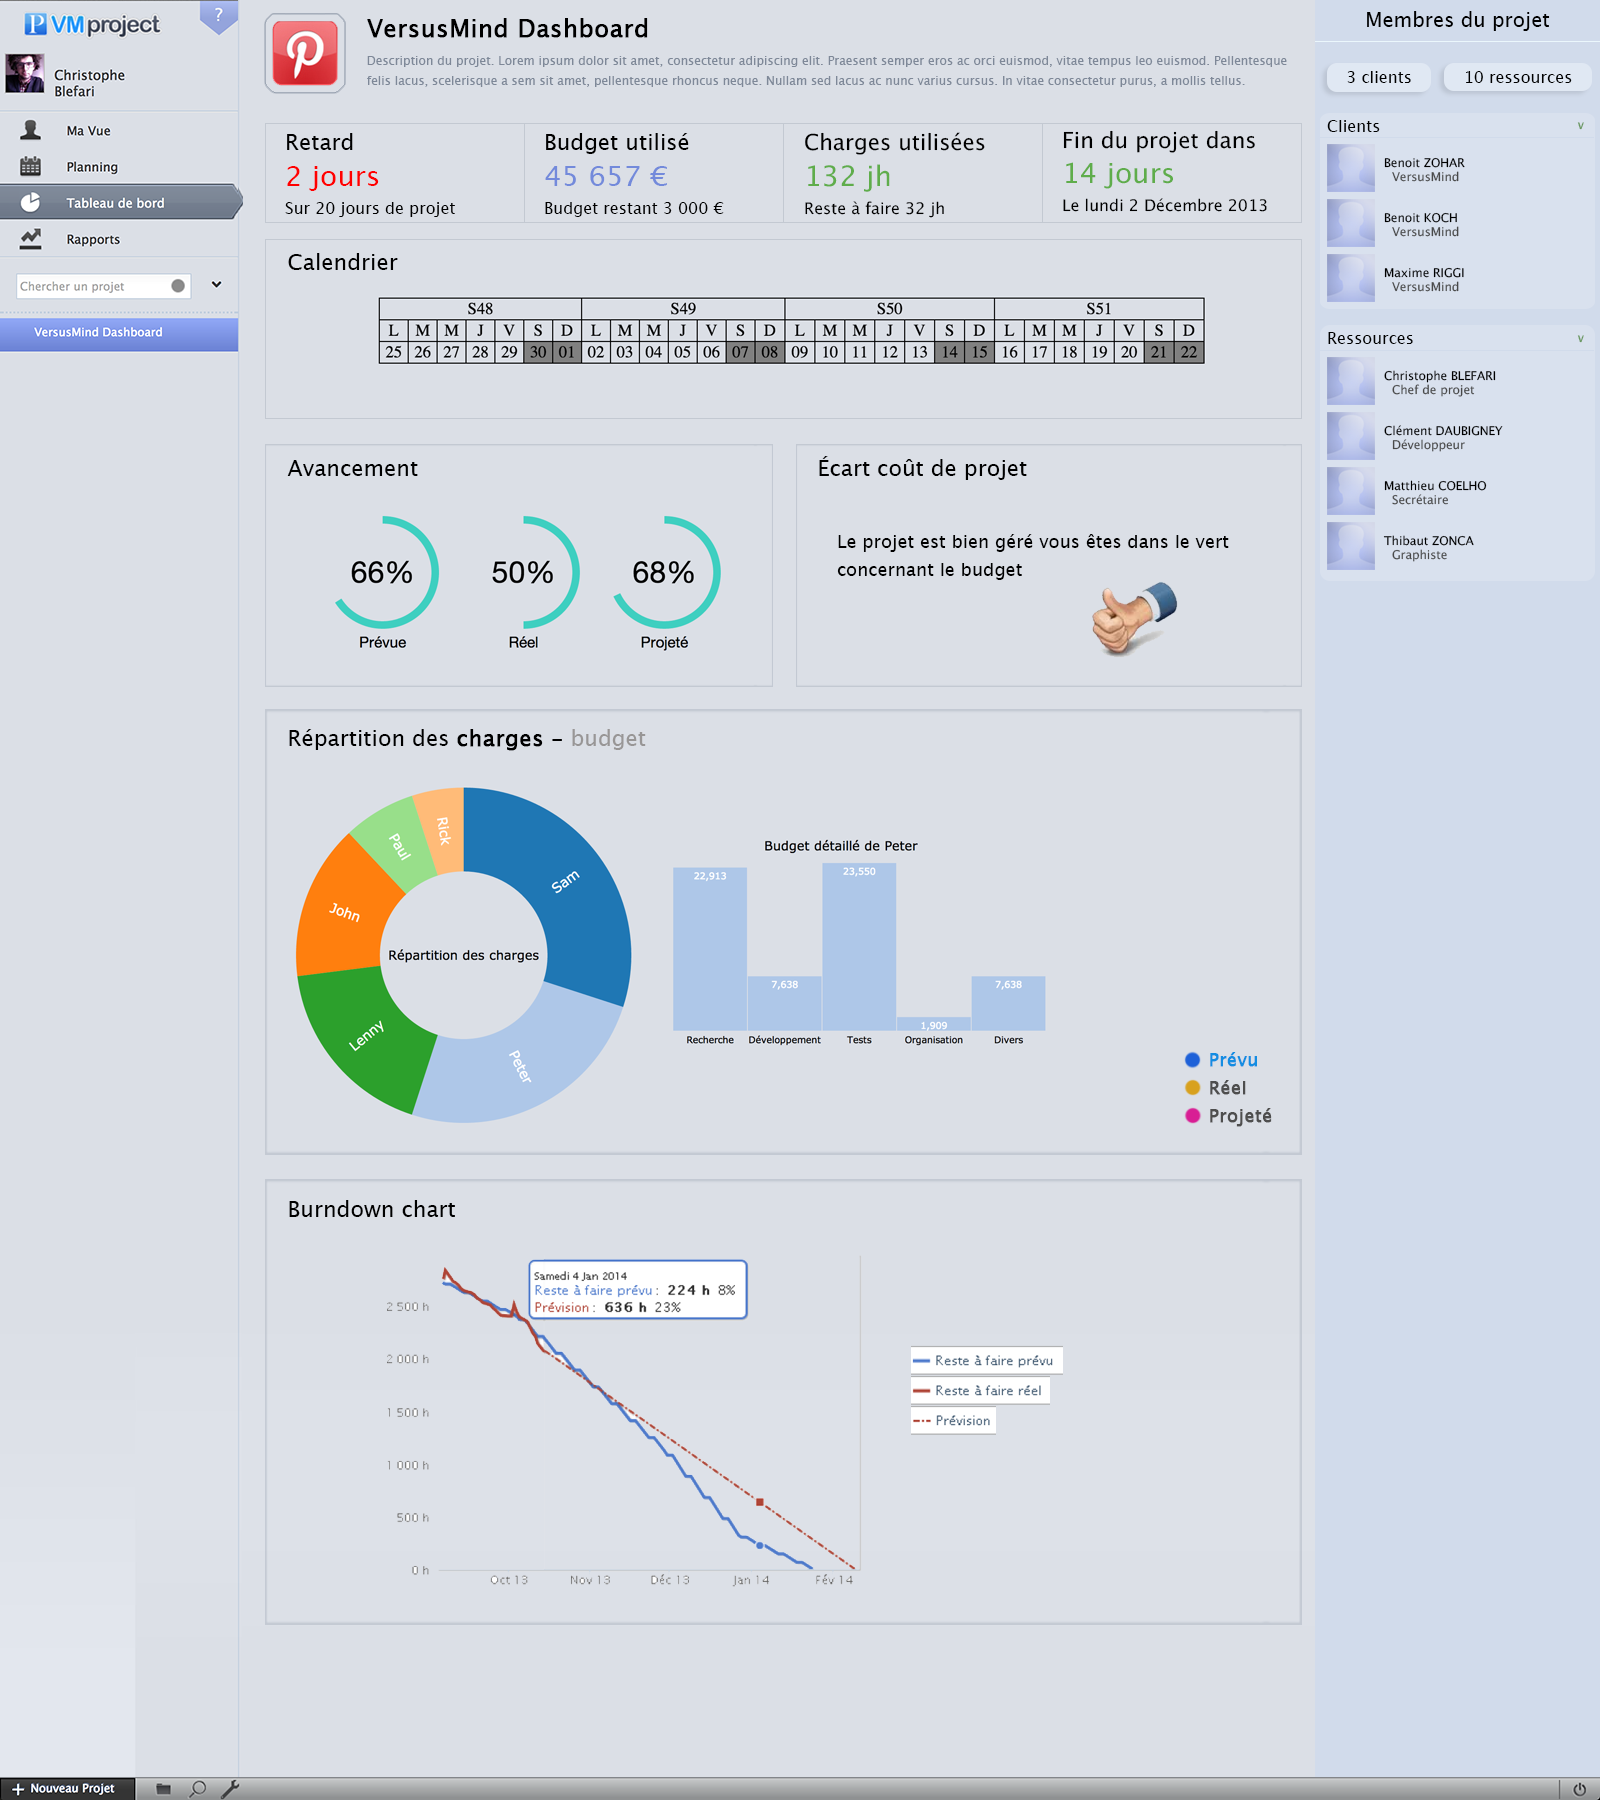
\includegraphics[width=1\textwidth]{pictures/maquettenous.png}
	\caption{Maquette réalisée sur Photoshop en conception}
	\label{a3}
\end{figure}
	
	\chapter{Maquette complète VersusMind}
	
	\begin{figure}[!h]
	\centering
	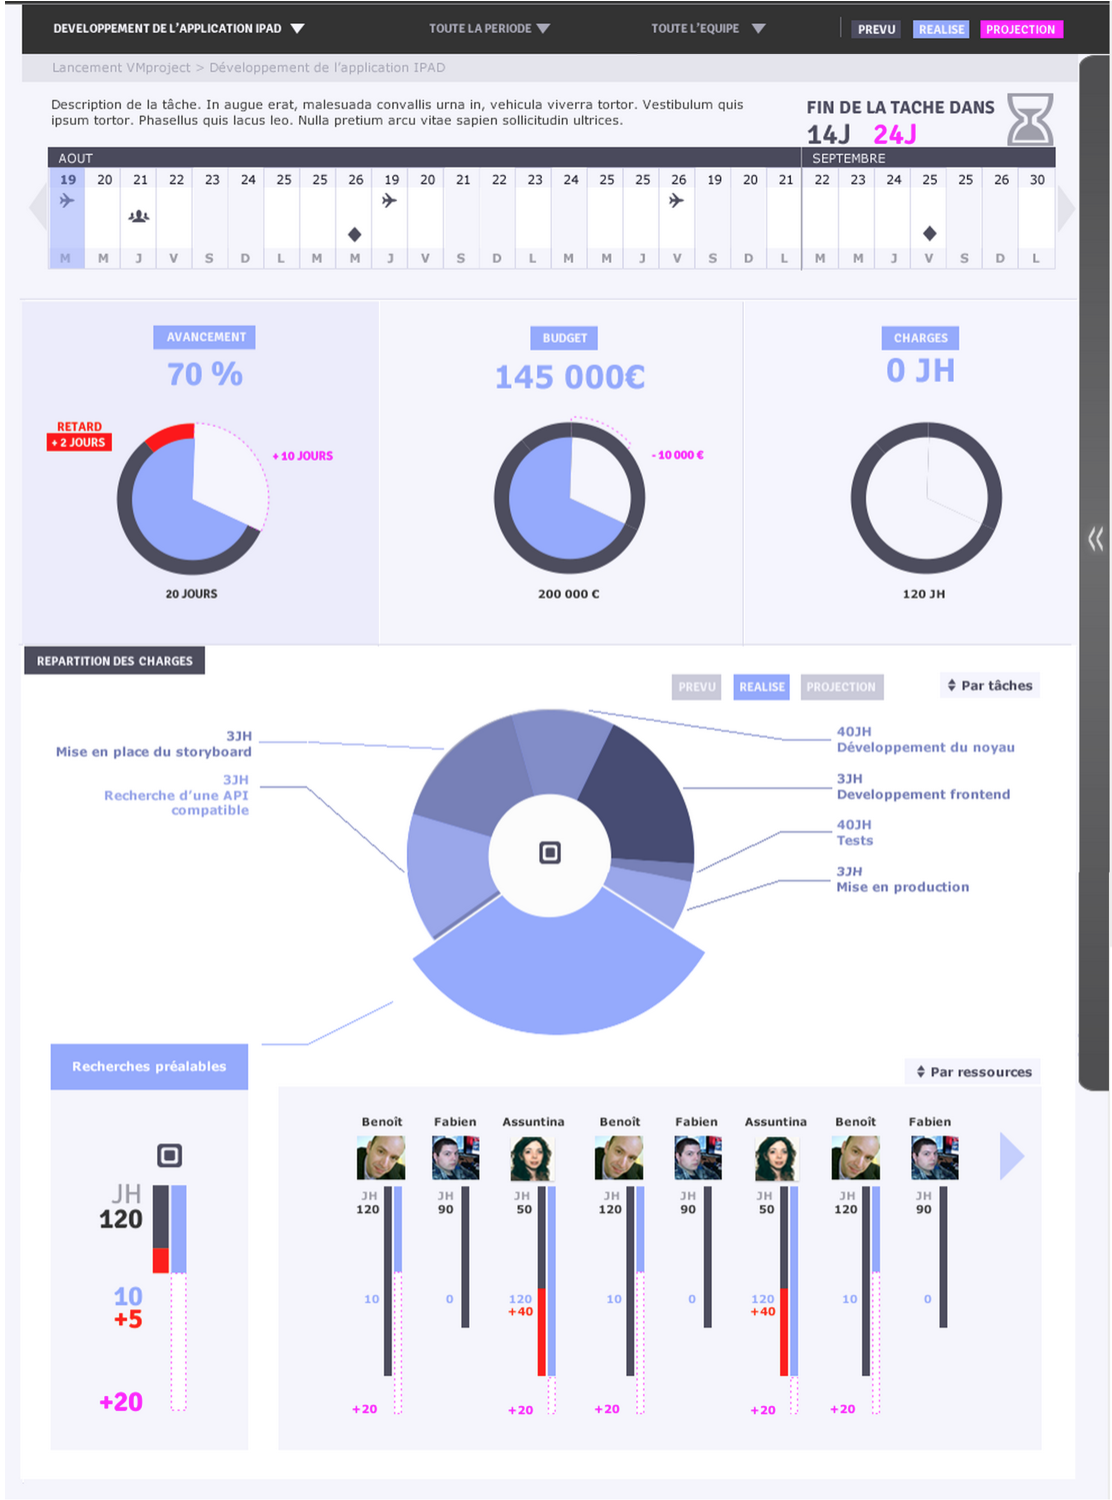
\includegraphics[width=0.9\textwidth]{pictures/maquetteeux.png}
	\caption{Maquette réalisée par Mme Gessa}
	\label{a4}
\end{figure}

\begin{figure}[H]
	\centering
	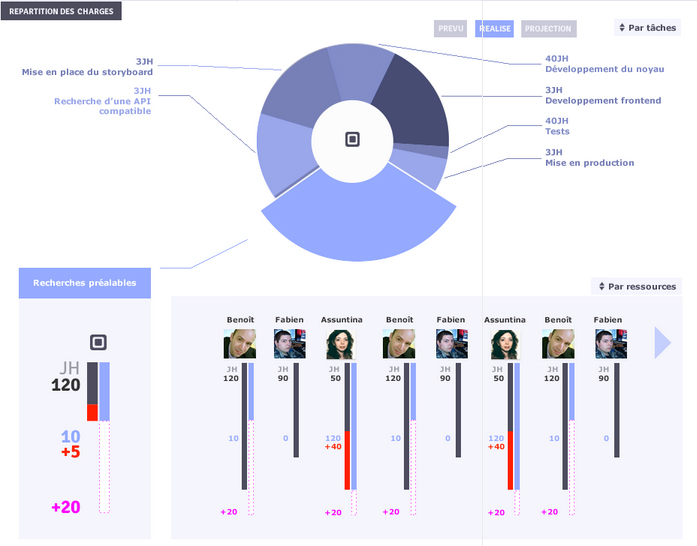
\includegraphics[width=1\textwidth]{pictures/maquetteVersusmind/repartitionClicked.jpg}
	\caption{Graphique de répartion, lorsqu'une part est cliquée}
	\label{15}
\end{figure}

Ici, une part (une tâche) a été cliquée et le détail de cette tâche est affiché en-dessous.\\

Sur la gauche, c'est le total des heures correspondant à cette tâche. Il ne faut pas forcément se fier aux nombres car la maquette qui nous a été renvoyée n'est pas aussi précise. Essayons de comprendre ce qui est affiché :\\

\begin{itemize}
\item Le nombre en bleu foncé correspond au prévu; cette tâche a donc été évaluée à 120 jours-hommes. Le rectangle bleu foncé à côté représente cette quantité de jours.
\item Le nombre en bleu clair, et sa représentation rectangulaire, correspondent au réel. Le rectangle réel étant plus grand que la barre prévue, on comprend que le chiffre réel est erroné. Il devrait en fait valoir 125.
\item Le nombre en rouge et le rectangle associé, correspondent au retard. C'est tout simplement la différence entre le réel et le prévu. Il vaut ici 5, ce qui est cohérent si le réel était bien de 125.
\item Enfin, le nombre et le rectangle rose correspondent au projeté. VMProject a donc calculé qu'il reste 20 jours-hommes de travail avant de terminer cette tâche, ce qui indique un retard total potentiel de 25 jours-hommes.\\
\end{itemize}

Sur la droite est présenté un niveau encore plus poussé de détails :\\

\begin{itemize}
\item Dans le cas où le camembert du haut était en mode "Par tâches", ce graphique présente au choix les tâches filles à la tâche cliquée, ou les ressources ayant travaillé sur tâche cliquée.
\item Si le camembert était en mode "Par ressources", le détail affiché ne porte que sur les tâches effectuées par la ressource cliquée (car nous n'allons pas afficher le détail par ressources d'une ressource).\\
\end{itemize}

La complexité de ce graphique nous a semblé au départ un peu déstabilisante mais elle a le mérite de présenter un maximum d'informations. Avec un petit temps d'adaptation, on peut comprendre ce graphique rapidement.\\

\begin{figure}[H]
	\centering
	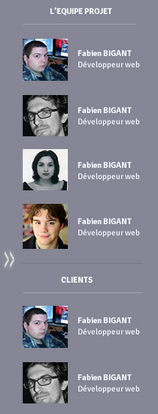
\includegraphics[width=0.3\textwidth]{pictures/maquetteVersusmind/barreMembres.jpg}
	\caption{Barre des membres du projet}
	\label{16}
\end{figure}
	
	\chapter{État de l'art librairie de charts}
	
	\begin{figure}[!h]
	\centering
	\includegraphics[width=0.45\textwidth]{pictures/comparatifcharts.png}
	\caption{Tableau comparatif des différentes lbrairies/framework de développement de graphiques}
	\label{a4}
\end{figure}
	
	\chapter{Vue avant impression}
	
	\begin{figure}[H]
	\centering
	\includegraphics[width=0.9\textwidth]{pictures/matthieu/m_imprimable.png}
	\caption{Vue d'impression}
	\label{m7}
\end{figure}

	\chapter{Implémentation des graphes indicateurs}
	
	\begin{figure}[H]
	\centering
	\includegraphics[width=0.9\textwidth]{pictures/clement/c3.png}
	\caption{Appel et différentes classes pour les trois "petits" graphes}
	\label{c3}
\end{figure}
La couleur bleue concerne la phase d’initialisation des graphes (arrivée sur la page) et les indications en vert décrivent le fonctionnement à chaque modification de sélecteur. \\
\end{appendices}


\end{document}